\documentclass[bibliography=totoc,listof=totoc,BCOR=5mm,DIV=12,oneside]{scrbook}

\usepackage[ngerman]{babel}
\usepackage[utf8]{inputenc}
\usepackage{graphicx}
\usepackage{url}
\usepackage[hidelinks]{hyperref}
\usepackage[natbib,style=apa,backend=biber]{biblatex}
\usepackage{csquotes}
\usepackage{amsmath}
\usepackage{lmodern}
\usepackage{inconsolata}
\usepackage[printonlyused]{acronym}
\usepackage{tocloft}
\usepackage{listings}
\usepackage{xcolor}

\definecolor{codegreen}{rgb}{0,0.6,0}
\definecolor{codegray}{rgb}{0.5,0.5,0.5}
\definecolor{codepurple}{rgb}{0.58,0,0.82}
\definecolor{backcolour}{rgb}{0.95,0.95,0.92}

\lstdefinestyle{mystyle}{
    backgroundcolor=\color{backcolour},
    commentstyle=\color{codegreen},
    keywordstyle=\color{magenta},
    numberstyle=\tiny\color{codegray},
    stringstyle=\color{codepurple},
    basicstyle=\ttfamily\footnotesize,
    breakatwhitespace=false,
    breaklines=true,
    captionpos=b,
    keepspaces=true,
    numbers=left,
    numbersep=1pt
}

\lstset{style=mystyle}

\graphicspath{{./Images/}}
\input{hyphenation}
\addbibresource{./Bibliography/bibliography.bib}

\urlstyle{tt}

\renewbibmacro*{doi+url}{
  \printfield{isbn}
  \newunit\newblock
  \iftoggle{bbx:doi}
    {\printfield{doi}
     \iffieldundef{doi}{}{\renewcommand*{\finentrypunct}{\relax}}}
    {}
  \newunit\newblock
  \iftoggle{bbx:url}
    {\usebibmacro{url+urldate}
     \iffieldundef{url}{}{\renewcommand*{\finentrypunct}{\relax}}}
    {}}

\setlength\cftparskip{-6pt}

\linespread{1.4}

\begin{document}
\sloppy

% ---------------------------------------------------------------
\frontmatter
    \thispagestyle{empty}
\cleardoublepage

\thispagestyle{empty}

\begin{center}

\vspace*{1cm}


\includegraphics[width=0.6\textwidth]{unibw_athene_logo}

\vspace{1.5cm}
{\Huge
\textbf{Hierarchisches Clustering von Kinect-Bewegungsdaten mittels Dynamic Time Warping}\\
}
\vspace{1.5cm}


{\Large
Bachelorarbeit von\\
Laurenz Fuchs\\
1196307\\
Draft vom \today % erleichtert die Zuordnung - für finale Version entfernen
}
\vspace{1cm}

\parbox{1cm}{
\begin{large}
\begin{tabbing}
Erstprüfer: \hspace{.5cm} \=Prof.\ Dr.\ Michael Koch\\[2mm]
Zweitprüfer: \>Prof.\ Dr.\ Gunnar Teege\\[2mm]
Betreuer:
\>M. Sc. Julian Fietkau\\[5mm]
Abgabetermin: \> 31. Mai 2022\\
\end{tabbing}
\end{large}}\\
\vspace{5mm}

\vfill

{\Large
Universität der Bundeswehr München\\
Fakultät für Informatik\\
}

\end{center}

    \thispagestyle{empty}
    \cleardoublepage
    \thispagestyle{empty}
    \cleardoublepage
    \vspace*{2cm}

\begin{center}
    \textbf{Kurzfassung}
\end{center}

\vspace*{1cm}

\noindent
Im Rahmen des \emph{HoPE-Projekts} wird das Verhalten von Menschen
bei der Nutzung von \emph{Ambient Displays} analysiert.
Tiefenkameras werden als eine mögliche Sensorik genutzt,
um Bewegungsabläufe aufzunehmen.
Konkret werden dazu Skelettdaten betrachtet.
Eine manuelle Analyse der Daten ist schwer umsetzbar.
Daher muss ein methodisches Rahmenwerk entwickelt werden,
welches eine Evaluation von Sensordaten ermöglicht.
Diese Bachelorarbeit ist ein Beitrag zu diesem Rahmenwerk.
Ziel ist die Entwicklung eines Java-Tools,
welches derartige Daten ohne Vorwissen, mithilfe deterministischer Algorithmen clustern kann.
Es kommt \emph{hierarchisches Clustering}
mittels des \emph{Dynamic Time Warping} Algorithmus zum Einsatz.
Es soll geklärt werden,
ob diese Algorithmen einen sinnvollen Beitrag zur Analyse von Bewegungsdaten leisten können.
Nach der Implementierung erfolgt ein Clustering von \emph{Kinect-Bewegungsdaten}.
Mithilfe einer Ground-Truth-Analyse und deskriptiven Statistiken
wird die Qualität der gefundenen Cluster überprüft.
Insbesondere hat hat sich dabei herausgestellt, dass ein geeigneter Threshold von großer Bedeutung ist.
Eine Evaluation bestätigt, dass die verwendeten Algorithmen zum Clustering
von Time-Series Daten genutzt werden können.
Für die Interpretation dieser Daten ist allerdings weitere Forschung notwendig.
    \thispagestyle{empty}
    \linespread{0.5}
    \tableofcontents
    \linespread{1.4}

% ---------------------------------------------------------------
\mainmatter

    \chapter{Einleitung}
\label{chapter1}
Von September 2021 bis August 2024 forschen die Hochschule für angewandte Wissenschaften Hamburg
und die Universität der Bundeswehr München im Rahmen des \emph{HoPE-Projekts} unter anderem am Verhalten
von Menschen bei der Nutzung von großen, interaktiven Wandbildschirmen.
Im Projekt wird unter anderem der \emph{Honeypot-Effekt} erforscht \citep{unibw_honeypot-effekt_2021}.
Dieser beschreibt in der \ac{HCI} wie Menschen, die mit einem System interagieren,
weitere Passanten anregen die Interaktion zu beobachten oder sogar an ihr teilzuhaben \citep{wouters_uncovering_2016}.
Der \emph{Honeypot-Effekt} soll bei der Nutzung von \emph{Ambient Displays} im öffentlichen
und halb-öffentlichen Raum in Langzeit-Feldstudien analysiert werden.
Dabei soll auch der Aspekt der Datenerhebung und -analyse weiter ausgebaut werden.
Hierzu muss ein methodisches Rahmenwerk entwickelt werden, welches eine auf Sensordaten-basierende,
automatische und zeitlich uneingeschränkte Evaluation von \emph{Ambient Displays} ermöglicht \citep{unibw_honeypot-effekt_2021}.
Die Sensordaten werden von Body-Tracking-Kameras bereitgestellt.
Es liegt ein Datensatz vor, bei dem Wandbildschirme mit Microsoft Kinect v2 Kameras ausgestattet wurden.
Diese zeichnen die Interaktion von Nutzern mit den Displays auf,
wodurch das Nutzerverhalten zu einem späteren Zeitpunkt ausgewertet werden kann.
Die Daten liegen als \emph{\ac{TSD}} vor.
Dabei handelt es sich um geordnete Sequenzen von Datenpunkten,
die über eine gewisse Zeit hinweg aufgenommen werden \citep{ali_clustering_2019}.
\emph{\ac{TSD}} enthalten oft wichtige Informationen, die durch eine Analyse entdeckt werden können \citep{ali_clustering_2019}.
Anhand dieser Informationen können die Daten gruppiert werden.
Dabei stellt sich die Frage, ob sich Kategorien identifizieren lassen,
die etwas über das Verhalten von Menschen vor Wandbildschirmen aussagen.
Wiederkehrende Bewegungsabläufe treten teilweise zu unterschiedlichen Zeitpunkten in den Aufnahmen auf.
Zudem kann sich die Ausführung bei verschiedenen Personen unterscheiden.
Dies erschwert eine manuelle Kategorisierung.
Bei großen Datensätzen ist eine manuelle Evaluation zur Beantwortung der Frage ohnehin nicht möglich.
Daher muss eine automatisierte Sortierung angeboten werden.
In dieser Bachelorarbeit wird versucht, dieses Problem mithilfe von deterministischen Algorithmen zu lösen.
Wesentliches Ziel ist die Implementierung eines Systems zur Kategorisierung der vorliegenden \emph{Kinect-Bewegungsdaten}.
Eine gängige Methode zur Analyse sind dabei \emph{Clustering}-Verfahren \citep{aghabozorgi_time-series_2015}.
Konkret soll \emph{hierarchisches Clustering} mithilfe des \emph{\ac{DTW}} Algorithmus eingesetzt werden.

Die Arbeit ist wie folgt aufgebaut:
Zunächst wird in \autoref{chapter2} auf wichtige Grundlagen der Thematik eingegangen.
Es werden mögliche Modelle der Interaktion mit Wandbildschirmen vorgestellt.
Außerdem werden die Grundzüge der Kinect Kamera und des vorliegenden Datensatzes dargestellt.
Abschließend erfolgt eine tiefergehende Erläuterung der Problemstellung.
\autoref{chapter3} widmet sich dem Hierarchischen Clustering und dem \ac*{DTW}-Algorithmus.
Gründe für die Wahl dieser Algorithmen werden hier erwähnt.
Nach einer ausführlichen Beschreibung der Funktionsweise
wird das Vorgehen an einem Beispiel veranschaulicht.
Am Ende wird auf verwandte Literatur
und den Einsatz im Kontext von Kinect-Bewegungsdaten eingegangen.
\autoref{chapter4} behandelt die Konzeption des Software-Tools.
Dafür werden die Anforderungen betrachtet,
bevor im Rest des Kapitels auf den geplanten Programmablauf,
sowie nötige Teilsysteme eingegangen wird.
Anschließend erfolgt die eigentliche Implementierung der Anwendung.
In \autoref{chapter5} wird deren Aufbau beleuchtet.
Außerdem werden zentrale Ausschnitte des Codes
und Abweichungen zur Konzeption beschrieben.
Abschließend erfolgt eine Evaluation (\autoref{chapter6}).
Hier wird zunächst auf Limitierungen der Anwendung
und die zur Evaluation verwendeten Daten eingegangen.
Teile des Datensatzes werden mithilfe des Tools geclustert.
Die Qualität der Cluster wird mithilfe von Ground-Truth Daten
und durch deskriptive Statistiken überprüft.
Ein abschließendes Fazit erfolgt in \autoref{chapter7}.
    \chapter{Grundlagen und Problembeschreibung}
\label{chapter2}
Bevor näher auf die verwendeten Algorithmen eingegangen wird,
werden grundlegende Aspekte erläutert.
Dabei werden neben einigen Interaktionsmodellen vor Wandbildschirmen
auch die eingesetzte Sensorik und die Struktur des Datensatzes beschrieben.
Zudem erfolgt abschließend eine ausführliche Problembeschreibung.


\section{Kategorien der Interaktion mit Wandbildschirmen}
\label{2-KategorienInteraktion-Wandbildschirme}
Interaktive digitale Medien sind in der Öffentlichkeit immer präsenter.
Deshalb wird es für Wandbildschirme immer schwieriger die Aufmerksamkeit von Passanten zu erregen
und sie zur Interaktion zu animieren.
Diese Herausforderungen können nicht einfach durch verbesserte Hardware oder attraktivere Displays gelöst werden.
Stattdessen muss ein besseres Verständnis von Menschen und deren Technologienutzung geschaffen werden \citep{wouters_uncovering_2016}.
\emph{Ambient Displays} sind große, interaktive Bildschirme im (halb-) öffentlichen Raum, mit denen Nutzer interagieren können.
Es handelt sich meist um ästhetisch ansprechende Displays die Personen mit Informationen versorgen \citep{mankoff_heuristic_2003}.
Eine Kategorisierung der Interaktion von Personen mit solchen Wandbildschirmen kann das Verständnis des Verhaltens verbessern.
Dazu existieren verschiedenste \emph{Audience Behaviour-Interaktionsmodelle}, wovon im Folgenden zwei näher beschrieben werden.

Das \emph{Audience Funnel Modell} beschreibt, wie Menschen sich um ein großes öffentliches Display versammeln
und von Beobachtern zu Interagierenden mit dem System, und anschließend wieder zu Beobachtern werden.
Menschen neigen dazu verschiedene Phasen der Interaktivität zu durchlaufen,
bevor sie direkt mit dem System interagieren \citep{wouters_uncovering_2016, mai_audience_2018}.
Die einzelnen Phasen des \emph{Audience Funnel} werden in \autoref{fig:AudienceFunnelModel} gezeigt.
Eine der Aufgaben eines Wandbildschirms ist es also Aufmerksamkeit auf sich zu ziehen
und den Nutzer zu motivieren mit dem System zu interagieren \citep{mai_audience_2018}.
\citet{mai_audience_2018} verweisen darauf, dass \emph{Ambient Displays} in der Öffentlichkeit
nicht undbedingt der zentrale Punkt der Aufmerksamkeit sind, da vorbeigehende Personen eigene intrinsische Ziele verfolgen.
Die Herausforderung für Entwickler ist es die Systeme so zu gestalten,
dass sie Aufmerksamkeit erregen, sich aber gleichzeitig nicht gezwungen in den Mittelpunkt stellen.

\begin{figure}[ht]
    \begin{center}
    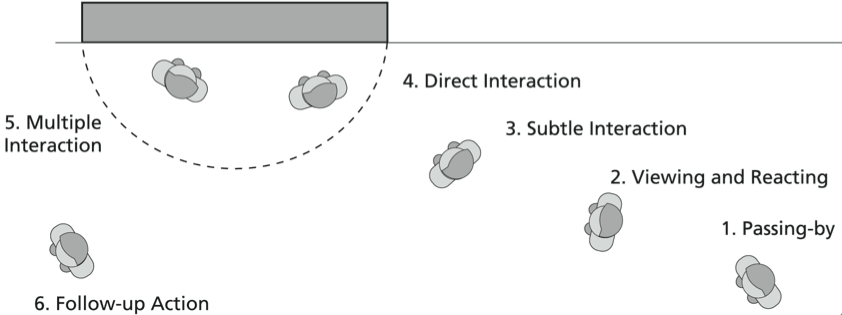
\includegraphics[width=0.9\textwidth]{audience-funnel-model.png}
    \end{center}
    \caption{Audience Funnel Framework. Abbildung aus \citet{mai_audience_2018}.}
    \label{fig:AudienceFunnelModel}
  \end{figure}

Ein zweites Modell wird durch den bereits erwähnten \emph{Honeypot-Effekt} beschrieben.
Er zeigt, dass Individuen undabhängig von Belohnungen, Bestrafungen oder sozialem Wettbewerb
von der reinen Präsenz oder den Aktivitäten anderer beeinflusst werden.
In der \ac{HCI} wird dies meist erkennbar, indem Passanten sich einem System nähern
und überlegen, ob sie mit ihm interagieren sollen,
nachdem sie anderen Menschen dabei zugesehen haben \citep{wouters_uncovering_2016}.

Eine Einordnung der Bewegungsdaten in die Kategorien solcher Modelle
und eine weiterführende Analyse der Bewegungen kann Aufschluss über das Verhalten von Menschen
vor interaktiven Bildschirmen geben.
Wie bereits erwähnt ist eine Kategorisierung des vorliegenden Kinect-Datensatzes
aufgrund der großen Datenmenge nicht manuell realisierbar.
Im Folgenden werden die Struktur des Datensatzes und die Grundlagen der verwendeten Sensorik beschrieben.
Aufbauend darauf werden Überlegungen angestellt,
wie eine Implementierung zur Automatisierung der Kategorisierung aussehen kann.


\section{Spezifikation der Kinect}
\label{2-SpezifikationKinect}
\citep{tolgyessy_evaluation_2021} verweisen darauf,
dass der Xbox 360 Kinect-Sensor eine \glqq Revolution\grqq\ im Bereich der erschwinglichen 3D-Erkennungssensorik war.
Ursprünglich war er für die Videospiel-Industrie gedacht.
Schon bald wurde er aber auch für wissenschaftliche Experimente genutzt.
In späteren Jahren folgten weitere Iterationen der Kinect \citep{tolgyessy_evaluation_2021}.
Im vorliegenden Datensatz des \emph{HoPE-Projekts} kam die Kinect v2 für Xbox One zum Einsatz.
Diese Sensorik stellt Farbbilder einer \ac{RGB} Kamera, Tiefenbilder einer Tiefenkamera
und Audiodateien verschiedener Mikrofone zur Verfügung \citep{windows-developer-center_microsoft_corporation_human_2014}.
Besonders die Tiefenkamera hilft zuverlässige Ergebnisse bei der Erkennung von Menschen vor \emph{Ambient Displays} zu erzielen.
\citet{li_time-flight_2014} fassen es wie folgt zusammen.
Die kompakte Größe, die Benutzungsfreundlichkeit,
die stark vereinfachte Hintergrund-Subtraktion im Vergleich zu anderer Sensorik, sowie die hohe Genauigkeit
und die hohe Bildrate machen Tiefenkameras zu einer attraktiven Lösung für ein breites Spektrum an Anwendungen.
Die Kinect v2 verwendet dabei den Ansatz der kontinuierlichen Wellenintensitätsmodulation,
der häufig bei \ac{ToF}-Tiefenkameras zum Einsatz kommt.
Dabei wird das Licht einer Lichtquelle von Objekten im Sichfeld der Kamera zurückgestreut
und die Phasenverzögerung zwischen dem emittierten und dem reflektierten Licht gemessen.
Diese Phasendifferenz wird für jedes Pixel im Bildfeld in einen Entfernungswert umgerechnet \citep{tolgyessy_evaluation_2021}.
Der Sensor kann Tiefenbilder mit einer Auflösung von 512 x 424 Pixeln
und gewöhnliche Farbbilder mit 1920 x 1080 Pixeln aufnehmen \citep{marin_multi-camera_2019}.
Bei der Kinect v2 können bis zu sechs Personen erfasst werden.
Dabei wird die Lage von 25 Skelettpunkten, sowie verschiedene Gesichtsattribute erfasst \citep{windows-developer-center_microsoft_corporation_human_2014}.
\autoref{fig:KinectBodyJoints} zeigt eine Übersicht dieser Punkte. 

\begin{figure}[ht]
  \begin{center}
  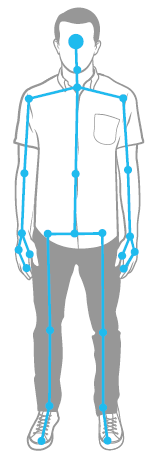
\includegraphics[width=0.1\textwidth]{kinect-body-joints.png}
  \end{center}
  \caption{Skelettpunkte der Kinect v2. Abbildung aus \citet{windows-developer-center_microsoft_corporation_human_2014}.}
  \label{fig:KinectBodyJoints}
\end{figure}


\section{Struktur des vorliegenden Datensatzes}
\label{2-StrukturDatensatz}
Zur Evaluation des implementierten System dienen verschiedene Teilmengen des Kinect-Datensatzes des \emph{HoPE-Projekts}.
Hierfür wurden im Jahr 2017 für 18 Wochen \emph{Ambient Displays} mit Kinect v2 Systemen ausgestattet.
Zu erwähnen ist zudem, dass das entwickelte Tool zur Auswertung auch mit anderen Datensätzen funktionieren soll.

Eine Auswertung des Datensatzes ergab, dass dieser 97.626 Records beinhaltet \citep{temiz_konzeption_2022}.
Dabei enthält jeder mehrere sogenannte Frames.
Dabei handelt es sich um Momentaufnahmen der Kinect-Sensorik.
Falls sich mehrere Menschen gleichzeitig im Sensorbereich befinden,
erhält jede Person eine eindeutige Identifikationsnummer
und der Record wird in mehrere Frames unterteilt.
Dabei entspricht ein Frame der Momentaufnahme einer Person.
Zu jedem Record liegen verschiedene Dateien vor,
die jeweils den Zeitstempel in Kombination mit einem geeigneten Postfix als Dateinamen tragen.
\autoref{tbl:AttributesDataset} zeigt die Attribute der Datei \emph{timestamp.txt}.
\begin{table}[ht]
  \begin{center}
    \begin{tabular}{ |c|c| } 
      \hline
      Attributname & Beschreibung \\
      \hline \hline
      Zeitstempel & Zeitpunkt der Aufnahme \\
      \hline
      KinectId & Skelett-Identifikationsnummer des Framework  \\
      \hline
      RecordId & Identifikationsnummer des Records \\
      \hline
      BodyIndex & Identifikationsnummer der Person \\
      \hline
      BodyCount & Anzahl der erfassten Personen \\
      \hline
      Happy & Person ist glücklich \\
      \hline
      Engaged & Person zeigt Interesse \\
      \hline
      WearingGlasses & Person trägt eine Brille \\
      \hline
      LeftEyeClosed & Person hat das linke Auge geschlossen \\
      \hline
      RightEyeClosed & Person hat das rechte Auge geschlossen \\
      \hline
      MouthOpen & Person hat den Mund geöffnet \\
      \hline
      MouthMoved & Person bewegt den Mund\\
      \hline
      LookingAway & Person schaut nicht zur Kinect \\
      \hline
      Body.HandLeftState & Zustand der linken Hand \\
      \hline
      Body.HandRightState & Zusand der rechten Hand \\
      \hline
      x & x-Koordinate des Skelettpunkts SpineShoulder \\
      \hline
      y & y-Koordinate des Skelettpunkts SpineShoulder \\
      \hline
      z & z-Koordinate des Skelettpunkts SpineShoulder \\
      \hline
      Distance & Distanz zwischen Kinect und Skelettpunkt SpineShoulder \\
      \hline
    \end{tabular}
    \caption{Attribute des Datensatzes.}
    \label{tbl:AttributesDataset}
  \end{center}
\end{table}
Diese Attribute werden in der Textdatei durch drei Rauten ('\#\#\#') voneinander abgegrenzt.
Ein konkreter Frame aus dem Datensatz kann \autoref{fig:FrameExample} entnommen werden.

\begin{figure}[ht]
  \begin{center}
    2017-04-10 07:41:53.943 +02:00 \#\#\# 72057594038063128 \#\#\# 1341053376 \#\#\# 
    \newline \#\#\# 1 \#\#\# 1 \#\#\# No \#\#\# Maybe \#\#\# Unknown \#\#\# No \#\#\# No \#\#\#
    \newline No \#\#\# Yes \#\#\# Maybe \#\#\# Unknown \#\#\# Closed \#\#\# 0,1074784
    \newline \#\#\# 0,2451882 \#\#\# 4,18441 \#\#\# 4,19296454679429
  \end{center}
  \caption{Frame aus dem Datensatz.}
  \label{fig:FrameExample}
\end{figure}

Da die Anordnung und das Vorhandensein dieser Attribute je nach Version des Datensatzes abweichen kann,
sollen diese in der Implementierung manuell konfigurierbar sein.
Die Datei \emph{timestamp$\_$bodies.txt} enthält für jeden Frame die Position aller 25 Skelettpunkte.
\emph{timestamp$\_$summary.txt} zeigt eine kurze Zusammenfassung des Records, welche gut menschenlesbar ist.
\emph{timestamp.xef} kann genutzt werden, um die Aufnahme in der Anwendung Kinect Studio zu visualisieren.
Letztlich sind die Einträge sogenannte \emph{\ac{TSD}}.
Bei diesem Datentyp handelt es sich um geordnete Sequenzen von Datenpunkten,
die über eine gewisse Zeit hinweg aufgenommen wurden.
Oft in regelmäßigen Abständen \citep{ali_clustering_2019}.
Insgesamt befinden sich im Datensatz 34.687.630 Frames \citep{temiz_konzeption_2022}.
Diese Anzahl bestätigt erneut die Notwendigkeit eines Software-Tools zur Auswertung.
Um aussagekräftige Ergebnisse zu erhalten lohnt es sich gegebenenfalls mit Teilmengen des Datensatzes zu arbeiten.
So liefern beispielsweise Records mit weniger als zwei Sekunden zu wenig Information
für Erkenntnisse über das Interaktionsverhalten.
Je nach Fragestellung kann es ebenfalls lohnenswert sein Records mit einer, zwei oder mehreren Personen
gesondert zu betrachten.

\section{Problembeschreibung}
\label{2-Problembeschreibung}
Es gibt verschiedene Möglichkeiten sich der Kategorisierung von Bewegungsdaten zu nähern.
So kann beispielsweise \emph{Maschine Learning} eingesetzt werden.
Dieser Ansatz wird derzeit ebenfalls im Rahmen des HoPE-Projekts erforscht \citep{plischke_master_2022}.
In dieser Bachelorarbeit werden hingegen \emph{deterministische Algorithmen} genutzt.
Durch sie kann die Implementierung eines Kategorisierungssystems verhältnismäßig einfach gehalten werden.
\citet{aghabozorgi_time-series_2015} verweisen zudem darauf, dass die Verwendung von Methoden
wie Maschine Learning (\emph{supervised}), im Falle von großen Datensätzen zu Problemen führen kann.
Deterministische Cluster-Algorithmen sollten bei großen Datenmengen weniger Probleme bereiten (\emph{unsupervised}).

Beim vorliegenden Kinect-Datensatz handelt es sich ebenfalls um eine große Datenmenge.
Die einzelnen Records müssen daher automatisiert bearbeitet werden.
Ziel der Verarbeitung ist es möglichst sinnvolle \emph{Cluster} zu erhalten.
Um die Gemeinsamkeiten zweier Aufnahmen zu berechnen,
wird eine geeignete Vergleichsfunktion benötigt.
Die Wahl dieser Funktion ist wichtig für den Erfolg des \emph{Clusterings} \citep{warren_liao_clustering_2005}.
Zu beachten ist zudem, dass die Bewegungsaufnahmen durch \emph{\ac{TSD}} beschrieben werden.
Werden hier herkömmliche Distanzmetriken, wie die Euklidische-Distanz verwendet
kann dies zu Problemen führen und die Aussagekraft des Vergleichs verringern.
Es kann vorkommen, dass verschiedene Personen die gleiche Bewegung unterschiedlich schnell,
oder zeitlich versetzt ausführen.
Gegebenenfalls weisen die Datenreihen bei der gleichen Bewegung daher sogar eine unterschiedliche Anzahl an Frames auf.
\autoref{fig:MetricComparison} zeigt ein exemplarisches Szenario.
Die Kurven weisen ähnliche Segmente auf.
Sie sind allerdings unterschiedlich lang und die Ähnlichkeiten treten zu unterschiedlichen Zeitpunkten auf.
Mit der bekannten euklidischen Distanz ist das Ergebnis hier nicht aussagekräftig
und der letzte Punkt der Reihe kann gar nicht zugordnet werden.
Um dieses Problem zu lösen ist eine elastische Metrik nötig,
die besser mit zeitlichen Verschiebungen umgehen kann \citep{aghabozorgi_time-series_2015}.

\begin{figure}[ht]
    \begin{center}
    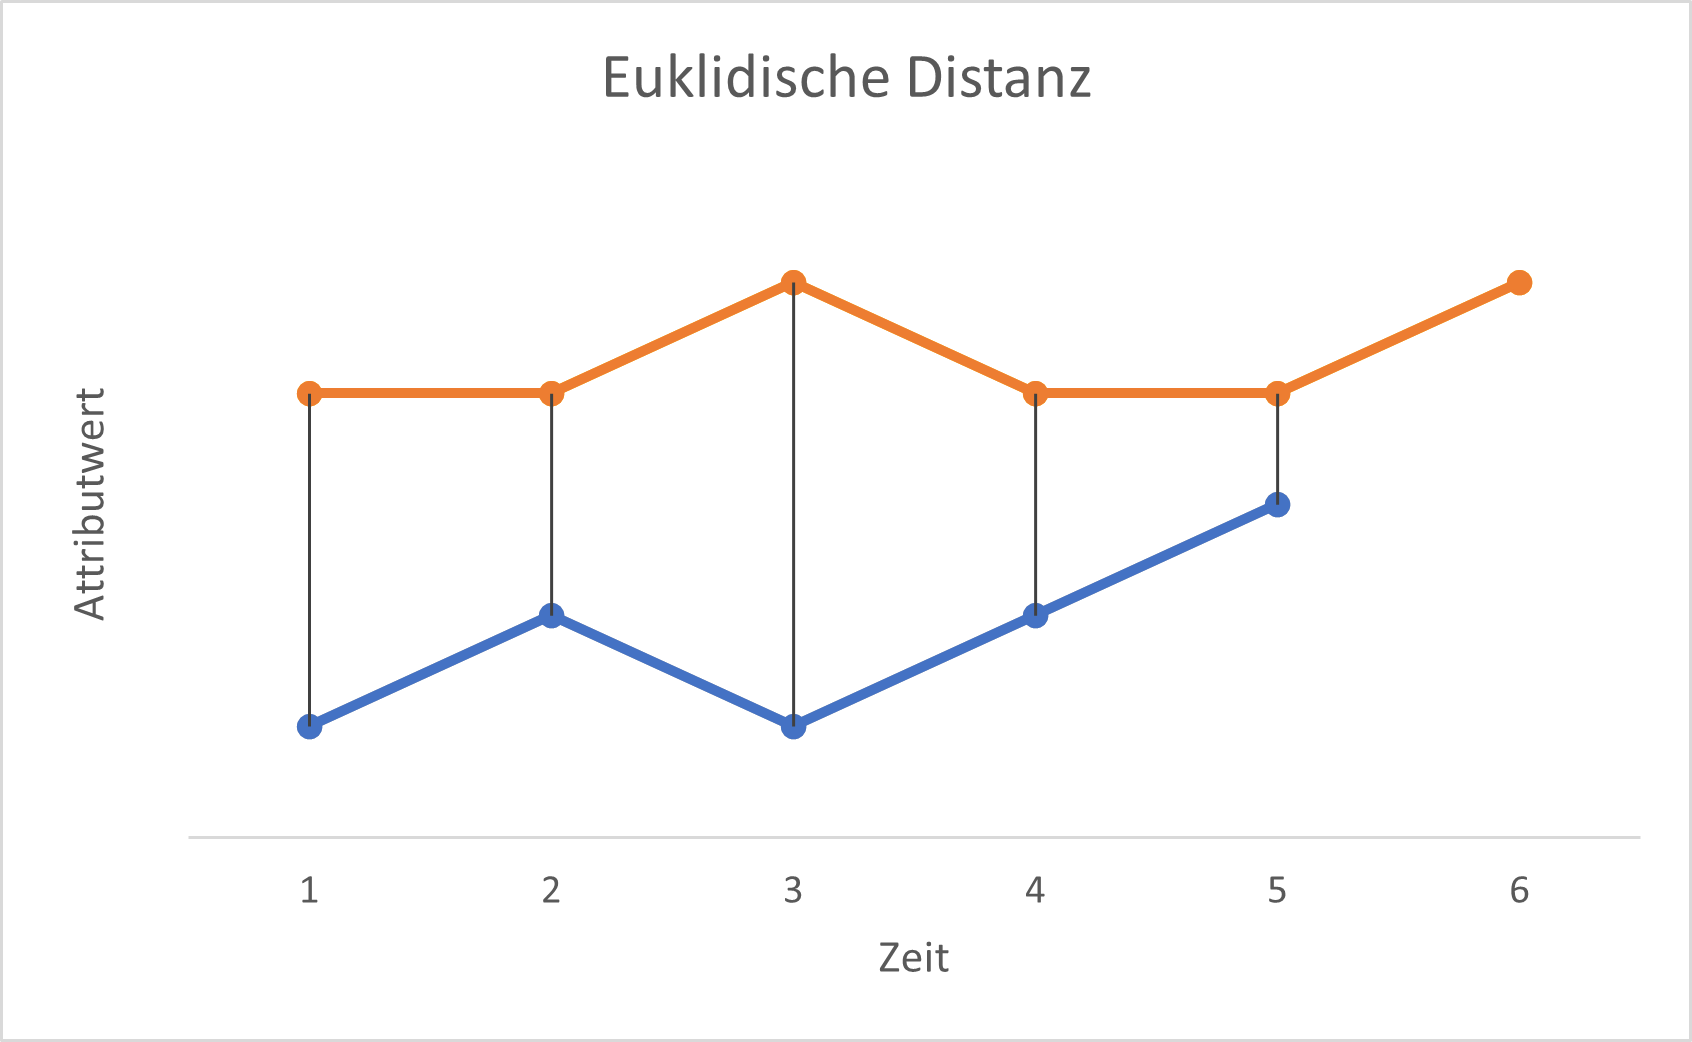
\includegraphics[width=0.45\textwidth]{EuclidianMetric.png}
    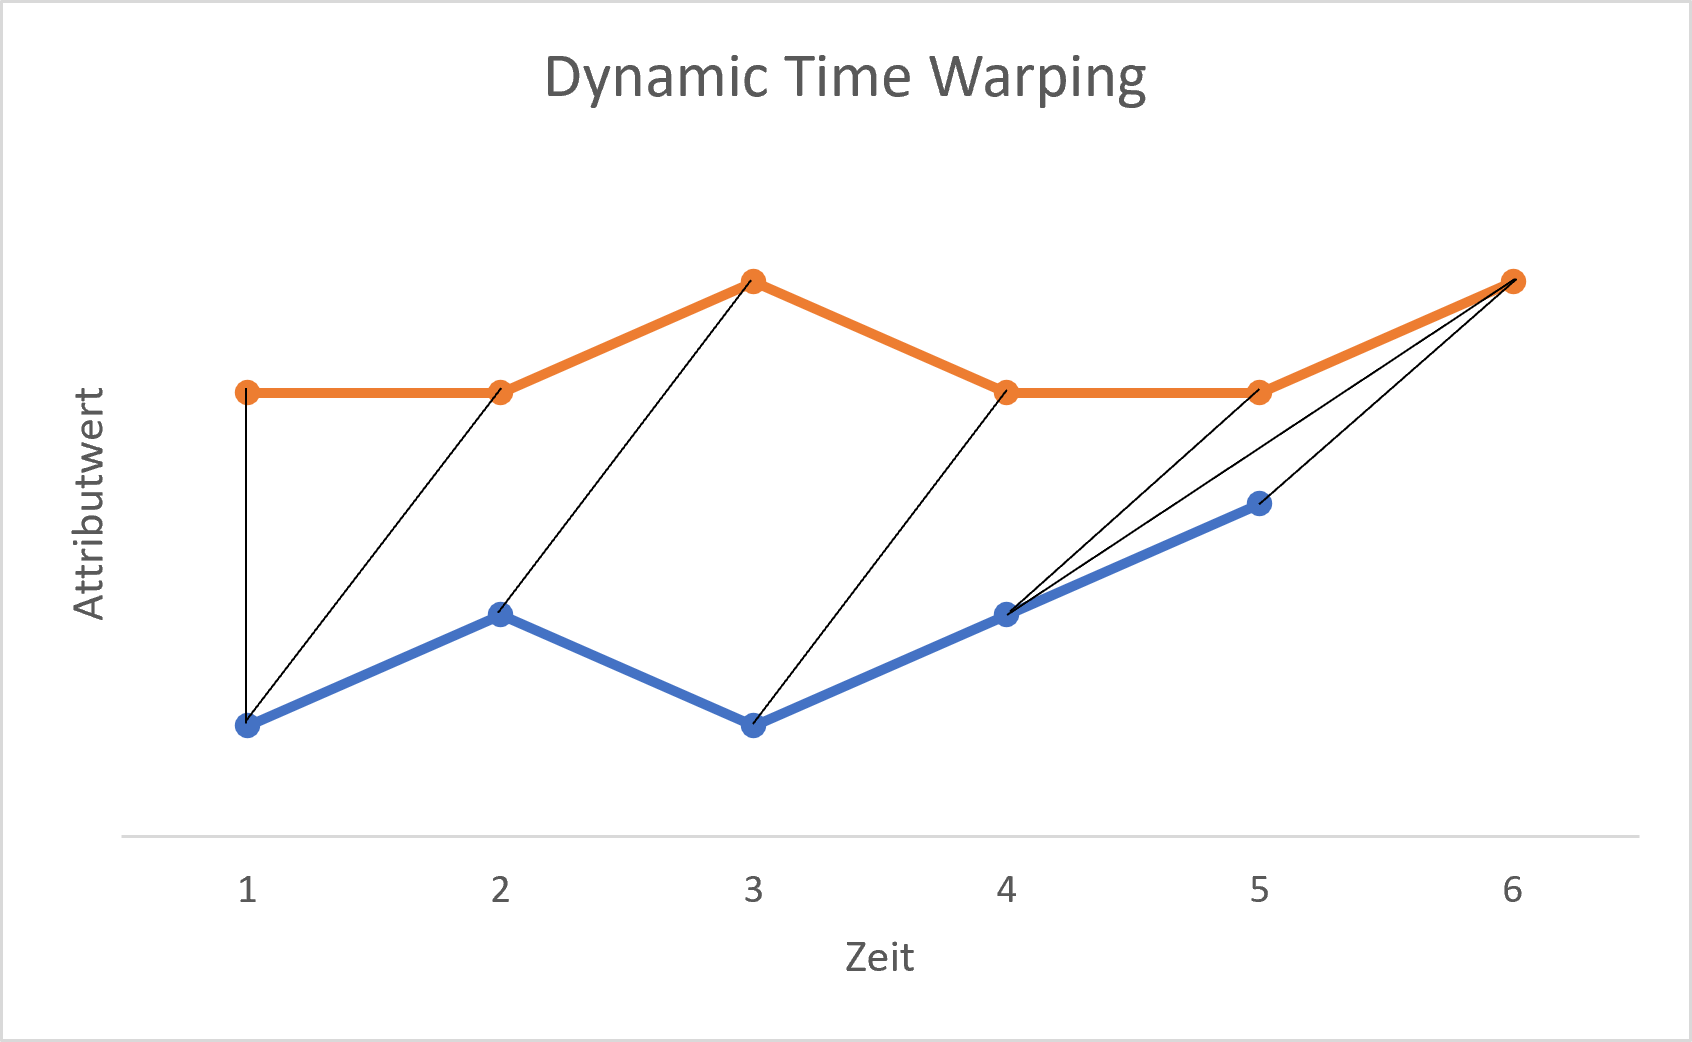
\includegraphics[width=0.45\textwidth]{DTWMetric.png}
    \end{center}
    \caption{Zuordnung der Messpunkte zweier Datenreihen.}
    \label{fig:MetricComparison}
\end{figure}

Das Clustering soll mithilfe von \emph{hierarchischem Clustering} durchgeführt werden,
welches in \autoref{3-Clustering} beschrieben wird.
Das Verfahren ist für die vorliegenden Daten gut geeignet,
da es erlaubt \ac{TSD} unterschiedlicher Länge zu clustern.
Zudem muss die Anzahl der zu bildenden Cluster nicht im Voraus definiert werden,
wie dies etwa bei \emph{K-Means} der Fall ist \citep{aghabozorgi_time-series_2015}.
Es ist in diesem Kontext nicht zielführend die Clusteranzahl zuvor zu definieren,
da die Arbeit darauf abzielt, mehr Erkenntnis über mögliche sinnvolle Cluster zu gewinnen.
Statt die Anzahl vorzugeben, wird ein Threshold definiert der angibt,
ab wann zwei Cluster nicht mehr zusammengeführt werden soll,
weil die Differenz zwischen ihnen zu groß ist.
Als geeignete Distanz-Metrik wird dabei \emph{\ac{DTW}} verwendet (\autoref{3-DTW}).
Hier ist eine Mehrfachzuordnung von Punkten möglich.
Diese können so verbunden werden, dass die Kosten minimal sind.
Dies erlaubt eine Zuordnung ähnlicher Muster in den Daten auch wenn sie zeitlich verschoben sind
und ist daher gut für unsere Problemstellung geeignet.
    \chapter{Konzeption}
\label{chapter3}


\section{Anforderungsanalyse}
\label{chapter3-Anforderungsanalyse}


\section{Programmablauf}
\label{chapter3-Programmablauf}


\section{Teilsysteme}
\label{chapter3-Teilsysteme}
    \chapter{Konzeption}
\label{chapter4}
Vor der eigentlichen Implementierung erfolgt nun die Konzeption.
Damit wird elaboriert, welche Anforderungen an die Software gestellt werden
und wie die Implementierung erfolgen muss.
Etwaige Ungereimtheiten und Probleme können so frühzeitig erkannt werden.

\section{Anforderungsanalyse}
\label{4-Anforderungsanalyse}
Es soll ein System implementiert werden,
welches Kinect-Bewegungsdaten mithilfe von hierarchischem Clustering
und \ac{DTW} als Distanzmetrik gruppiert.
Es gibt sogenannte \emph{funktionale Anforderungen} und \emph{nicht-funktionale Anforderungen},
die das System erfüllen muss.
Letztere beinhalten beispielsweise Anforderungen zu Benutzbarkeit, Effizienz oder Portierbarkeit.
Funktionale Anforderungen beschreiben hingegen die primären Funktionen des Systems.
Im Austausch mit Mitarbeitern des HoPE-Projekts haben sich die folgenden Anforderungen ergeben.

\subsection{Nicht-funktionale Anforderungen}
\label{4-NichtFunktionaleAnforderungen}
Das Tool soll ohne großen Installationsaufwand nutzbar sein
und daher, nach Möglichkeit, eine stark verbreitete Programmiersprache nutzen.
Bei der Implementierung fällt deshalb die Wahl auf Java in der Version 14.
Um weitere Installationen zu vermeiden sollen auch keine externen Bibliotheken genutzt werden.
An die Effizienz gibt es keine besonderen Anforderungen,
da die Auswertung der Daten nur einmalig erfolgt.
Eine Echtzeitauswertung ist also nicht geplant.
Zu lange Wartezeiten, schränken allerdings die Nutzbarkeit des Tools ein.
Daher sollen berechnete Kosten in einer geeigneten Datenstruktur zwischengespeichert werden.
So können im darauffolgenden Iterationsschritt Berechnungsschritte eingespart werden.
Des Weiteren soll das Tool durch wenige Anpassungen auch auf Datensätze anderer Tiefenkameras angewandt werden können.
Um dieses Ziel zu erreichen, wird die Software von Beginn an generisch entwickelt.
Zu allen Bestandteilen des Tools existiert daher ein Interface.
Bei Bedarf können so mit wenig Aufwand neue Implementierungen,
die den Anforderungen anderer Datensätze entsprechen, ergänzt werden.

\subsection{Funktionale Anforderungen}
\label{4-FunktionaleAnforderungen}
Die Anwendung sollte die folgenden Funktionalitäten anbieten.
Unter anderem ist sie für den Input zuständig.
Ein Datensatz kann aus Textdateien eingelesen und in passenden Datenobjekten abgespeichert werden.
Das Tool soll ein Clustering mittels hierarchischem Clustering wie in \autoref{3-Clustering} beschrieben anbieten.
Dabei ist der Threshold für das Mergen von zwei Clustern vom Nutzer konfigurierbar.
Als Distanzmetrik wird \ac{DTW} (\autoref{3-DTW}) genutzt.
Des Weiteren ist konfigurierbar, welche Attribute des Datensatzes für den Vergleich genutzt werden.
Zur Berechnung der Distanz zwischen zwei Punkten wird die euklidische Distanz verwendet.
Allerdings können hier weitere Funktionen ergänzt werden.
Mit Hilfe eines Startparameters kann entschieden werden, welche dieser Funktionen für die Berechnung verwendet wird.
Zudem besitzt das Tool Output-Funktionalitäten.
Die gefundenen Cluster werden in einer Textdatei aufgelistet.
Jedes Cluster erhält eine eindeutige Identifikationsnummer und eine Liste aller Records, die zusammengeführt wurden.
Für ein erleichtertes Verständnis der Cluster wird auch eine primitive Visualisierung der Cluster angeboten.
Die starke Konfigurierbarkeit wird durch eine \emph{config-file} erreicht,
die der Nutzer beim Start der Anwendung übergeben kann.
\autoref{tbl:AttributesConfig} zeigt deren Attribute.
\begin{table}[ht]
    \begin{center}
        \begin{tabular}{ |c|c| } 
            \hline
            Attributname & Beschreibung \\
            \hline \hline
            inputPath & Pfad zum Datensatz. \\
            \hline
            outputPath & Pfad zum Ablegen der Output-Dateien.  \\
            \hline
            separator & Trennzeichen zwischen den Attributen. \\
            \hline
            datasetType & Art des vorliegenden Datensatzes. \\
            \hline
            threshold & Grenzwert für das Zusammenführen von Clustern. \\
            \hline
            attributes & Vorhandene Attribute. \\
            \hline
            usedAttributes & Attribute, die zum Vergleich genutzt werden. \\
            \hline
            distanceFunction & Bezeichnung der genutzten Distanzfunktion. \\
            \hline
            flipVisualization & Wahrheitswert, ob die Visualisierung gespiegelt wird. \\
            \hline
            attributeForBodyIdentification & Bezeichnung des Körperidentifikationsparameters. \\
            \hline
            skipFrames & Wahrheitswert, ob jeder dritte Frame ignoriert wird. \\
            \hline
        \end{tabular}
        \caption{Attribute der Configuration-Datei.}
        \label{tbl:AttributesConfig}
    \end{center}
\end{table}

\section{Teilsysteme}
\label{4-Teilsysteme}
\autoref{fig:Packages} kann das Paketdiagramm des Tools entnommen werden.
Das Paket \emph{model} enthält sowohl die Interfaces für Cluster, Records und Frames,
als auch jeweils geeignete Implementierungen für den Kinect-Datensatz.
Bei Bedarf können hier bei späterer Verwendung der Software weitere Implementierungen
für andere Datensätze ergänzt werden.
Im \emph{utility}-Paket befinden sich Interfaces für Reader und Writer.
Auch hier sind geeignete Implementierungen bereitgestellt.
Ein Reader für die Config-Datei, ein Reader für die Kinect-Daten
und ein Writer für die gefundenen Cluster.
Auch das Interface und die Implementierung für die Visualisierung befinden sich hier.
Im Paket \emph{calculating} befinden sich alle Klassen die für das Clustern der Daten benötigt werden.
Es ist weiter untergliedert in \emph{clustering} und \emph{metric}.
Letzteres liefert die Vergleichsmetrik für unser Clusterverfahren.
Wieder liegen geeignete Interfaces vor,
sodass die Anwendung bei Bedarf um weitere Metriken oder Clustering-Ansätze erweitert werden kann.
Bereitsgestellt werden initial eine Implementierung mit hierarchischem Clustering
und \ac{DTW} als Metrik.
Das Paket \emph{processor} ist von zentraler Bedeutung,
denn hier wird die Funktionalität des Tools zusammengeführt.
Zunächst werden die benötigten Reader Instanzen initialisiert.
Mit ihnen werden die Daten eingelesen.
Anschließend wird das Clustering gestartet.
Die Ergebnisse werden in der Ausgabedatei gespeichert und zusätzlich visualisiert.
\begin{figure}[ht]
    \begin{center}
    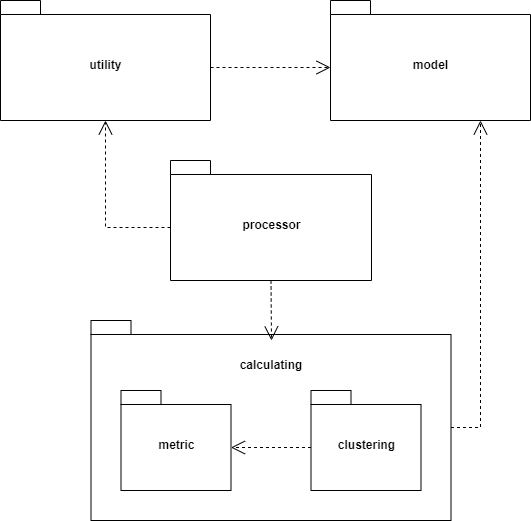
\includegraphics[width=0.9\textwidth]{packages.png}
    \end{center}
    \caption{Paketdiagramm des Tools.}
    \label{fig:Packages}
\end{figure}

\clearpage
\section{Programmablauf}
\label{4-Programmablauf}
Im Folgenden wird der Programmablauf beschrieben.
\begin{enumerate}
    \item Der Nutzer startet den \emph{Clustering-Processor}
    und gibt als Startparameter den Pfad der \emph{config-Datei} an.
    \item Der \emph{Processor} nutzt den \emph{Config-Reader}, um die Werte der \emph{Konfigurationdatei} auszulesen
    und speichert diese ab.
    \item Der \emph{Processor} nutzt den \emph{DataReader}, um den Datensatz einzulesen
    und legt die Informationen in geeigneten Objekten ab.
    Beim Kinect-Datensatz sind das die Implementierungen \emph{RecordImpl} und \emph{FrameImpl}
    der entsprechenden Interfaces.
    \item Der \emph{Processor} startet das Clustering durch den Aufruf der \emph{cluster-Methode}
    eines \emph{HierarchicalClustering-Objekts}.
    Zu beginn entspricht jeder Record einem eigenen Cluster.
    Die \emph{recordToCluster-Methode} ermöglicht eine Transformation.
    \item Das Clustering nutzt ein \emph{\ac{DTW}-Objekt},
    um paarweise die Kosten zweier Cluster zu berechnen.
    \item Die beiden Cluster mit den geringsten Kosten werden zusammengeführt.
    Konkret wird eines der Cluster in das andere integriert.
    Dadurch entsteht eine Kombination beider Cluster.
    Beim integrierten wird ein boolescher Wert auf \emph{false} gesetzt,
    damit das Cluster in späteren Berechnungsschritten nicht mehr beachtet wird.
    Dabei wird jeweils das Mittel der Attributwerte berechnet und abgelegt.
    Zudem werden die Cluster-Bestandteile abgespeichert.
    Bei allen Komponenten wird ebenfalls der boolesche Wert auf \emph{false} gesetzt,
    damit sie bei zukünftigen Vergleichen nicht mehr berücksichtigt werden.
    \item Schritte 5 und 6 werden so lange wiederholt, bis die geringsten Kosten den vom Nutzer definierten Threshold übersteigen.
    \item Der \emph{Processor} nutzt den \emph{Cluster-Writer}, um alle Cluster der \emph{clusters-Liste}
    in eine Ausgabedatei zu schreiben.
    \item Der \emph{Processor} nutzt die \emph{VisualizerImpl}, um alle Records der gefundenen Cluster zu visualisieren.
    \item Die Anwendung terminiert. 
\end{enumerate}

    \chapter{Implementierung}
\label{chapter5}
Wie bereits erwähnt erfolgt die Implementierung mit Java.
Damit für die Nutzung keine weiteren Installationen nötig sind,
werden nur die Java-Standardbibliotheken zur Umsetzung genutzt.
Der gesamte Source Code kann unter \href{https://github.com/lzfs/tsprocessor}{github.com/lzfs/tsprocessor}
abgerufen werden.
In diesem Kapitel wird vertiefend auf die Struktur des Tools eingegangen.
Zudem werden wichtige Aspekte der Implementierung betrachtet.

\section{Aufbau}
\label{5-Aufbau}
Der detailierte Aufbau des Tools kann dem Klassendiagramm in \autoref{fig:Classes} entnommen werden.
Dabei wurde aus Gründen der Übersichtlichkeit auf Konstruktoren,
Getter- und Setter-Methoden verzichtet.
\begin{figure}[p]
    \begin{center}
        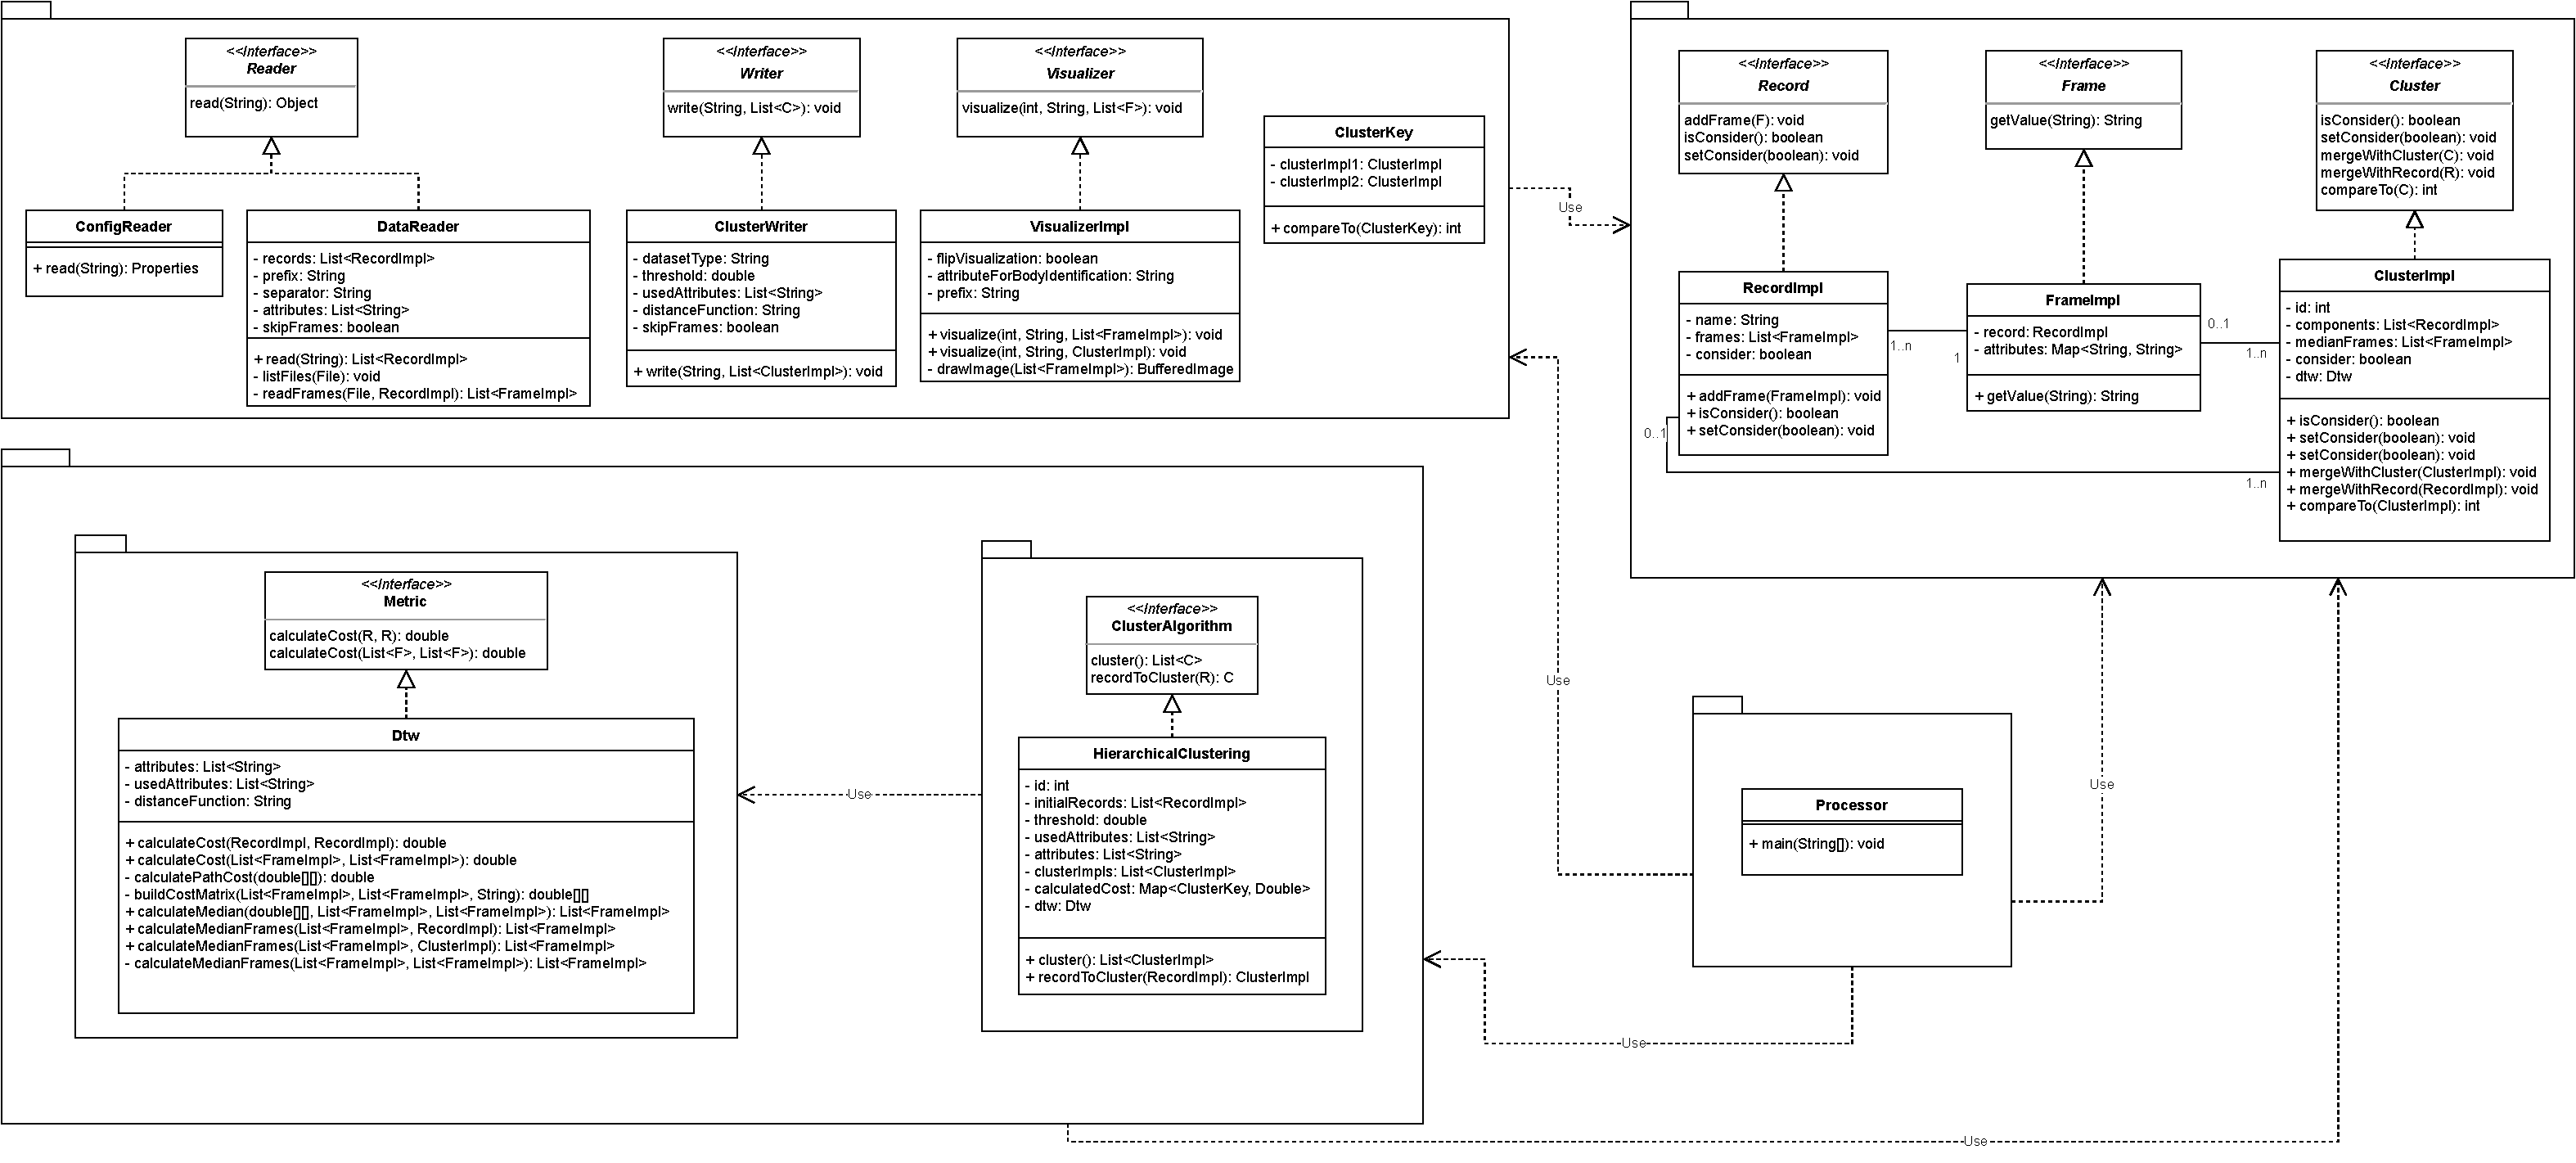
\includegraphics[width=1.3\textwidth, angle=90]{classes.pdf}
    \end{center}
    \caption{Klassendiagramm des Tools.}
    \label{fig:Classes}
\end{figure}
Die wichtigsten Aspekte der Software werden im Folgenden beschrieben.
Die grobe Struktur entspricht der aus \autoref{4-Teilsysteme}.
Zum Start der Anwendung ist ein Aufruf der \emph{main-Methode} des \emph{Processor} nötig.
Dieser initialisiert zunächst geeignete \emph{Reader}.
Das \emph{Reader-Interface} wird von den Klassen \emph{ConfigReader} und \emph{DataReader} implementiert.
Der \emph{ConfigReader} dient lediglich dazu, die Werte der Config-Datei einzulesen.
Dabei wird ein \emph{Properties-Objekt} zurückgeliefert,
mit dem auf die jeweiligen Werte zugegriffen werden kann.
Der DataReader liest die Kinect-Daten ein.
Ihm wird zunächst übermittelt, welche Attribute vorhanden sind,
durch welches Zeichen sie voneinander abgetrennt sind
und ob Frames übersprungen werden sollen,
um die Performanz zu verbessern.
Mit diesen Informationen können die Daten geeignet eingelesen und eine \emph{RecordImpl-Liste} zurückgeliefert werden.
Jede \emph{RecordImpl} enthält dabei eine Liste von \emph{FrameImpls}.
Diese Datentypen sind die entsprechenden Implementierungen der Interfaces \emph{Record} und \emph{Frame}.
Sie können für Kinect-Daten genutzt werden.
Eine FrameImpl enthält jeweils eine Map mit ihren Attributen,
welche mithilfe der \emph{getValue-Methode} abgerufen werden können.
Der letzte Datentyp ist das Cluster und die zugehörige \emph{ClusterImpl}.
Cluster bestehen aus beliebig vielen, aber mindestens einer RecordImpl.
Die Bestandteile werden in einer Liste gespeichert.
Hier werden die Methoden \emph{mergeWithCluster} und \emph{mergeWithRecord} angeboten.
Mit ihnen wird jeweils eine weitere Komponente in die ClusterImpl integriert.
ClusterImpls haben außerdem eine eindeutige Identifikationsnummer und eine Liste der berechneten
\emph{FrameImpl-Mittelwerte} aller Komponenten.
Zudem besitzen sie, genau wie die RecordImpls, einen Wahrheitswert, der angibt,
ob die ClusterImpl in zukünftigen Kombinationsschritten weiterhin beachtet werden soll.
Alle genannten Interfaces können bei Bedarf geeignet für andere \ac{TSD}-Datensätze implementiert werden.
Nach dem Einlesen und Abspeichern der Daten startet der Processor das Clustering.
Dazu wird eine Instanz von \emph{HierarchicalClustering}, einer Implementierung von \emph{ClusterAlgorithm}, erstellt.
Das Objekt erhält dafür alle wichtigen Informationen,
wie die initialen RecordImpls, den Threshold und die Attribute vom Processor.
Da jede ClusterImpl am Anfang aus einer einzigen RecordImpl besteht,
wird die Methode \emph{recordToCluster} angeboten.
Mit ihr kann jeder der initialen RecordImpls transformiert
und anschließend in der \emph{clusterImpl-Liste} abgelegt werden.
Die \emph{cluster-Methode} kümmert sich um den eigentlichen Cluster-Vorgang.
Dabei nutzt sie zur Berechnung von Kosten eine Instanz der \emph{Dtw-Klasse}.
Sie implementiert das \emph{Metric-Interface} und bietet daher die nötigen Methoden,
um die Kosten zwischen zwei RecordImpls, beziehungsweise deren \emph{FrameImpl-Listen} zu berechnen.
Dabei kommt der in \autoref{3-DTW} beschriebene \ac{DTW}-Algorithmus zum Einsatz.
Um auch eine ClusterImpl mit einer RecordImpls vergleichen zu können bietet die Klasse zudem entsprechende
\emph{calculateMedianFrames-Methoden}, die aus mehreren \emph{FrameImpl-Listen} eine neue erzeugt,
indem die Werte mithilfe von \ac{DTW} kombiniert werden.
Das genaue Verhalten der Klassen HierarchicalClustering und \emph{Dtw} wird in \autoref{5-Codebeschreibung} näher betrachtet.
Nach dem Ende der Berechnungen liegen die gefundenen ClusterImpls in der \emph{clusterImpl-Liste} vor.
Sie werden mit dem \emph{ClusterWriter} geeignet in einer Textdatei abgespeichert.
Zudem erfolgt eine Visualiserung mithilfe der \emph{VisualizerImpl}.
Die Klasse nutzt dazu Java-AWT-Komponenten.
Der Wahrheitswert \emph{flipVisualization} gibt dabei an,
ob die Werte in x-Richtung gespiegelt werden sollen.
Dies ist nötig, da bei der Kinect das Koordinatensystem aus Nutzersicht erstellt wird.
In der Visualiserung führt dies dazu, dass die aufgezeichneten Bewegungen spiegelverkehrt erscheinen.
Der String \emph{attributeForBodyIdentification} dient dazu,
die unterschiedlichen Personen im Record korrekt darzustellen.

\section{Codebeschreibung}
\label{5-Codebeschreibung}
Nach der Beschreibung des Ablaufs und der groben Struktur
sollen nun wichtige Codeausschnitte des hierarchischen Clusterings
und des \ac{DTW} Algorithmus beschrieben werden.
Objekte der Klassen ClusterImpl, RecordImpl und FrameImpl werden in diesem Abschnitt
vereinfacht als Cluster, Record und Frame bezeichnet.
Bei der Ausführung des folgenden Codes wurden die Daten bereits eingelesen.
Zudem wurde ein HierarchicalClustering-Objekt mit den nötigen Parametern erzeugt.
Damit wird die cluster-Methode gestartet.
Die Klasse HierarchicalClustering verfügt über eine clusterImpl-Liste,
welche zunächst leer ist.
Sie wird mit den initialen Clustern belegt,
indem alle Records zunächst zu trivialen Clustern transformiert werden
und anschließend der Liste hinzugefügt werden.
Des Weiteren werden die nötigen Variablen für die Berechnung deklariert.
\autoref{lst:ClustInit} zeigt diese Schritte.
Der eigentliche Berechnungsablauf wird in \autoref{lst:ClustCalc} gezeigt.
Er befindet sich in einer Schleife, die mindestens einmal ausgeführt wird.
Sie wird so lange fortgesetzt, bis die geringsten gefundenen Kosten den Threshold übersteigen,
oder nur noch ein einziges Cluster übrig ist.
Die Merge-Kandidaten geben die Indizes der beiden Cluster mit den
geringsten Kombinationskosten an.
In jedem Durchlauf der while-Schleife werden die Werte der Kosten
und die gewählten Merge-Kandidaten zurückgesetzt.
Dazu werden standardmäßig das erste und zweite Cluster in der Liste und deren Kosten gewählt.
Im Anschluss werden mittels der geschachtelten Schleifen paarweise die Cluster miteinander verglichen.
Dabei werden nur Cluster, deren \emph{consider-Wert} noch \emph{true} ist, in Betracht gezogen.
Außerdem darf es sich beim Vergleich nicht zweimal um das gleiche Cluster handeln.
Mithilfe der \emph{calculatedCost-Map} wird geprüft, ob die Kosten für diese Kombination schon berechnet wurden.
Falls nicht, werden sie neu berechnet.
Als Schlüssel dient ein Objekt der \emph{ClusterKey-Klasse}.
Deren \emph{equal-Methode} ist so definiert,
dass \emph{new ClusterKey(clusterImpl1, clusterImpl2).equals(new ClusterKey(clusterImpl2, clusterImpl1)) == true} gilt.
Somit wird auch der symmetrische Fall beachtet.
Immer wenn eine Kombination gefunden wird, deren Kosten geringer sind als die bisherigen,
wird die aktuelle Belegung der Minimalkosten und der Merge-Kandidaten angepasst.
Nach dem Vergleich aller Cluster, erfolgt die Kombination der beiden mit den geringsten Kombinationskosten.
Dies ist in \autoref{lst:ClustMerge} zu sehen.
Die Indizes der beiden Cluster mit den geringsten Kombinationskosten sind
in \emph{mergeCandidate1} und \emph{mergeCandidate2} abgelegt.
Die zugehörigen Kosten sind in der Variablen \emph{currentMinimumCost} abgelegt.
Sind diese immer noch geringer als der definierte Threshold, können die Kandidaten zusammengeführt werden.
Dazu wird \emph{mergeCandidate2} mit der Methode \emph{mergeWithCluster} in \emph{mergeCandidate1} integriert.
Dabei wird der \emph{consider}-Wert des \emph{mergeCandidate2}-Clusters auf \emph{false} gesetzt,
da es in künftigen Schritten nicht mehr als eigenständige Einheit betrachtet werden soll.
Abschließend müssen alle berechneten Werte mit \emph{cluster1} aus der \emph{calculateCost-Map} entfernt werden,
da die aktuellen Werte aufgrund der neuen Komponente nicht mehr gültig sind.
Die Kosten mit \emph{cluster2} können ignoriert werden, da diese Cluster ohnehin nicht mehr betrachtet werden.
In den oben gezeigten Clustering-Schritten wurden die Kosten mithilfe der \emph{calculateCost-Methode} berechnet.
\autoref{lst:DtwCalc} zeigt diese.
Für jedes der Attribute, das für die Berechnung verwendet werden soll, wird gemäß des \ac{DTW}-Algorithmus
eine Kostenmatrix aufgestellt (\autoref{lst:DtwMatrix}).
Für sie werden die minimalen Pfadkosten berechnet und zu den Gesamtkosten für diesen Attributvergleich addiert.
Das Ergebnis wird am Ende durch die Anzahl der betrachteten Attribute dividiert,
um auch vergleichbare Werte zu erhalten, wenn die Anzahl von Attributen variiert.
Die Methode \emph{buildCostMatrix} liefert die passende Kostenmatrix für ein gemeinsames Attribut
zweier Frame-Listen gemäß des \ac{DTW}-Algorithmus.
Zunächst werden die beiden Attributreihen in Arrays kopiert.
Anschließend wird die initiale Matrix erstellt.
Die Zellen der Reihe und Spalte mit dem Index \emph{0} werden mit dem Wert {\glqq unendlich\grqq} belegt.
Die Zelle \emph{(0, 0)} und alle übrigen Zellen erhalten den Wert 0.
Nun werden die Attributwerte paarweise verglichen.
Hier wird standardmäßig die absolute Distanz verwendet.
Bei Bedarf können an dieser Stelle weitere Distanzmetriken ergänzt werden.
Zur berechneten Differenz wird jeweils das Minimum der angrenzenden, bereits berechneten Zellen addiert.
Diese Summe wird in die entsprechende Matrixzelle eingetragen.
Dadurch füllt sich die Matrix und kann nach Abschluss der Berechnungen zurückgegeben werden.
Die Kosten des Warping Pfads der entsprechenden Matrix können mithilfe der Methode \emph{calculatePathCost}
berechnet werden.
Das Verfahren startet in der letzten Zelle der Matrix und sucht den Pfad mit den geringsten Kosten,
um die Zelle \emph{(0, 0)} zu erreichen.
Dabei werden die in \autoref{3-DTW} beschriebenen Vorgaben eingehalten.
Die Kosten des Pfades werden aufsummiert und anschließend durch die Anzahl der betretenen Zellen geteilt.
Diese Division ist nötig, um, im Falle von unterschiedlich großen Matrizen, vergleichbare Ergebnisse zu erhalten.
\autoref{lst:DtwPath} veranschaulicht dieses Vorgehen.
\begin{lstfloat}
\begin{lstlisting}[language=Java, label={lst:ClustInit}, caption=Cluster-Methode: Initialisierung.]
  // Initialize each record as a cluster and add it to the clusters list.
  for (RecordImpl record : this.initialRecords) {
      this.clusterImpls.add(this.recordToCluster(record));
  }
  double currentMinimumCost;
  double cost;
  int mergeCandidate1;
  int mergeCandidate2;
\end{lstlisting}
\end{lstfloat}
\begin{lstfloat}
    \begin{lstlisting}[language=Java, label={lst:ClustCalc}, caption=Cluster-Methode: Berechnungsvorgang.]
    do {
      // Reset for next loop iteration.
      cost = this.dtw.calculateCost(    
          this.clusterImpls.get(0).getMedianFrames(),
          this.clusterImpls.get(1).getMedianFrames());
      currentMinimumCost = cost;
      mergeCandidate1 = 0;
      mergeCandidate2 = 1;
      for (ClusterImpl clusterImpl1 : this.clusterImpls) {
          for (ClusterImpl clusterImpl2 : this.clusterImpls) {
              if (
                  clusterImpl1 != clusterImpl2
                  && clusterImpl1.isConsider()
                  && clusterImpl2.isConsider()) {
                  if (this.calculatedCost.containsKey(
                      new ClusterKey(clusterImpl1, clusterImpl2))) {
                      cost = this.calculatedCost.get(
                          new ClusterKey(clusterImpl1, clusterImpl2));
                  }
                  else {
                      cost = this.dtw.calculateCost(
                          clusterImpl1.getMedianFrames(),
                          clusterImpl2.getMedianFrames());
                      this.calculatedCost.put(
                          new ClusterKey(clusterImpl1, clusterImpl2), cost);
                  }
                  if (cost < currentMinimumCost) {
                      /* If a cost smaller than the current minimum cost
                      has been found it will be the new minimum. */
                      currentMinimumCost = cost;
                      mergeCandidate1 = this.clusterImpls.indexOf(clusterImpl1);
                      mergeCandidate2 = this.clusterImpls.indexOf(clusterImpl2);
                  }
              }
          }
      }
      // Merging. Showed in next Listing.
    } while (currentMinimumCost < threshold && this.clusterImpls.size() > 1);
\end{lstlisting}
\end{lstfloat}
\begin{lstfloat}
\begin{lstlisting}[language=Java, label={lst:ClustMerge}, caption=Cluster-Methode: Mergevorgang.]
  if (currentMinimumCost < threshold) {
      /* MergeCandidate1 and mergeCandidate2 should be merged together.
      Merge cluster2 into cluster1 and update the cluster list.
      Consider of cluster2 is set to false. */
      this.clusterImpls.get(mergeCandidate1).mergeWithCluster(
          this.clusterImpls.get(mergeCandidate2));  
      this.clusterImpls.remove(this.clusterImpls.get(mergeCandidate2));
      // Create a copy of the map to avoid an exception.
      Map<ClusterKey, Double> calculatedCostCopy = new HashMap<>(calculatedCost); 
      /* Remove all calculated costs from the map that contain
      cluster1 because it changed and therefore all cost values
      with this cluster have to be calculated again. */
      for (Map.Entry<ClusterKey, Double> entry : calculatedCostCopy.entrySet()) {
          /* Ignore mergeCandidate2 because it got removed from the list and
          the consider value of cluster2 is set to false. */
          if (entry.getKey().getCluster1().getId() == mergeCandidate1
                || entry.getKey().getCluster2().getId() == mergeCandidate1) {
              for (ClusterImpl clusterImpl : clusterImpls) {
                  calculatedCost.remove(
                      new ClusterKey(
                          this.clusterImpls.get(mergeCandidate1), clusterImpl));
              }
          }
      }
  }
\end{lstlisting}
\end{lstfloat}
\begin{lstfloat}
\begin{lstlisting}[language=Java, label={lst:DtwCalc}, caption=DTW: Berechnung der Kosten.]
  public double calculateCost(
      List<FrameImpl> frames1,
      List<FrameImpl> frames2) {
      // Add the calculated cost of each attribute to it.
      double cost = 0;
      // Calculate the cost for all attributes.
      for (String attribute : this.usedAttributes) {
          // Build the cost matrix for this attribute.
          double[][] dtwMatrix = buildCostMatrix(frames1, frames2, attribute);
          // Calculate and add the cost of this attribute.
          cost += calculatePathCost(dtwMatrix);
      }
      return cost / this.usedAttributes.size();
  }
\end{lstlisting}
\end{lstfloat}
\begin{lstfloat}
\begin{lstlisting}[language=Java, label={lst:DtwMatrix}, caption=DTW: Kostenmatrix.]
  private double[][] buildCostMatrix(
      List<FrameImpl> frames1,
      List<FrameImpl> frames2,
      String attribute) {
      double[] s = new double[frames1.size()];
      double[] t = new double[frames2.size()];
      int counter = 0;
      for (FrameImpl frame : frames1) {
          s[counter] = Double.parseDouble(frame.getValue(attribute));
          counter += 1;
      }
      counter = 0;
      for (FrameImpl frame : frames2) {
          t[counter] = Double.parseDouble(frame.getValue(attribute));
          counter += 1;
      }
      int n = s.length;
      int m = t.length;
      // Filled with zeros by default.
      double[][] dtwMatrix = new double[n + 1][m + 1];
      for (int i = 0; i < dtwMatrix.length; i++) {
          for (int j = 0; j < dtwMatrix[0].length; j++) {
              // Filled with infinity by definition of dtw.
              dtwMatrix[i][j] = Double.POSITIVE_INFINITY;
          }
      }
      // Filled with zero by definition of dtw.
      dtwMatrix[0][0] = 0;
      for (int i = 1; i < dtwMatrix.length; i++) {
          for (int j = 1; j < dtwMatrix[0].length; j++) {
              double cost = Math.abs(s[i - 1] - t[j - 1]);
              double minTmp = Math.min(dtwMatrix[i - 1][j], dtwMatrix[i][j - 1]);
              double lastMin = Math.min(minTmp, dtwMatrix[i - 1][j - 1]);
              dtwMatrix[i][j] = cost + lastMin;
          }
      }
      return dtwMatrix;
  }
\end{lstlisting}
\end{lstfloat}
\begin{lstfloat}
\begin{lstlisting}[language=Java, label={lst:DtwPath}, caption=DTW: Warping Path berechnen.]
  public double calculatePathCost(double[][] dtwMatrix) {
      int n = dtwMatrix.length - 1;
      int m = dtwMatrix[n - 1].length - 1;
      int pathCounter = 1;
      double cost = dtwMatrix[n][m];
      while (n != 0 && m != 0) {
          double minTmp = Math.min(dtwMatrix[n - 1][m], dtwMatrix[n][m - 1]);
          double lastMin = Math.min(minTmp, dtwMatrix[n - 1][m - 1]);
          cost += lastMin;
          if (lastMin == dtwMatrix[n - 1][m - 1]) {
              n = n - 1;
              m = m - 1;
          }
          else if (lastMin == dtwMatrix[n - 1][m]) {
              n = n - 1;
          }
          else if (lastMin == dtwMatrix[n][m - 1]) {
              m = m - 1;
          }
          pathCounter += 1;
      }
      return cost / pathCounter;
  }
\end{lstlisting}
\end{lstfloat}

\clearpage
\section{Abweichungen zur Konzeption}
\label{5-AbweichungenKonzeption}
Alle im folgenden genannten Punkte waren in der ursprünglichen Konzeption nicht vorgesehen.
Die Notwendigkeit der Anpassungen wird im Folgenden begründet.

An die Performanz der Anwendung wurden keine besonderen Anforderungen gestellt
(\autoref{4-NichtFunktionaleAnforderungen}).
Es zeigte sich aber schnell, dass bereits Datensätze mit einigen Hundert Records zu langen Bearbeitungszeiten führen.
Daher wurden zwei Konzepte umgesetzt, die sich diesem Problem annehmen.
Zum einen werden die berechneten Kosten in einer Map abgespeichert,
um wiederholte Berechnungen in darauffolgenden Schritten zu vermeiden.
Als Key der jeweiligen Map-Einträge dient ein Objekt der Klasse ClusterKey.
Sie implementiert das Comparable-Interface und sorgt dafür,
dass zwei Cluster zusammen als Key einer Map verwendet werden können.
Dies spart viele Berechnungsschritte,
da beinahe alle Werte im Vergleich zum vorherigen Iterationsschritt gleichbleiben.
Lediglich jene Kosten, an denen die neu zusammengeführten Cluster beteiligt waren,
sowie die Kosten mit dem neuen Cluster müssen neu berechnet werden.
Zum anderen gibt es die Möglichkeit jeden dritten Frame der Records zu ignorieren.
Dies geschieht, indem der Parameter \emph{skipFrames} in der config-Datei auf \emph{true} gesetzt wird.
Damit ist in der Regel weiterhin ein sinnvolles Clustering möglich,
wobei die Anzahl der Berechnungsschritte reduziert werden kann.
Es ist zu erwähnen, dass es dabei zu einem Informationsverlust kommt.
Diese Option sollte daher nur bei Bedarf genutzt,
wenn ansonsten beispielsweise der Zeitaufwand für die Berechnung zu hoch ist.

Zudem wurde abweichend zur Konzeption ein primitiver Visualizer ergänzt,
da sonst die Analyse der Cluster manuell über Kinect Studio erfolgen muss.
Er stellt die Laufwege der gefundenen Cluster aus der Vogelperspektive dar.
Für jedes Cluster wird ein Verzeichnis erstellt.
Darin werden die einzelnen Komponenten visualisiert.
    \chapter{Evaluation}
\label{chapter6}
Um die Praxistauglichkeit zu überprüfen, werden nun ausgewählte Daten
mithilfe des entwickelten Tools geclustert.
Die Ergebnisse werden anschließend bewertet.
Zur Bewertung des Clusterings werden \emph{externe}
und \emph{interne} Indizes unterschieden \citep{aghabozorgi_time-series_2015, warren_liao_clustering_2005}.
Bei einem \emph{externen Index} werden \emph{Ground-Truth-Daten} extern bereitgestellt.
Nach dem Clustering kann der Grad der Übereinstimmung zwischen gefundenen Clustern
und den vorgegebenen Clustern überprüft werden \citep{aghabozorgi_time-series_2015, warren_liao_clustering_2005}.
Die Daten werden mithilfe einer Visualisierung manuell geclustert.
In \autoref{6-GroundTruth} werden die gefundenen Cluster mit den erwarteten verglichen.
Bei \emph{internen Indizes} muss die Qualität der Cluster hingegen
ohne zusätzliche Informationen überprüft werden \citep{aghabozorgi_time-series_2015, warren_liao_clustering_2005}.
Dazu sollen in \autoref{6-Statistical} \emph{deskriptive Statistiken} genutzt werden.
Die Standardabweichung, der Mittelwert, das Maximum und das Minimum liefern
ein Maß für die Ähnlichkeit von Cluster-Komponenten.
Damit wird überprüft,
ob zusammengefasste Records tatsächlich einen hohen Grad an Übereinstimmung aufweisen.

\section{Einführende Bemerkungen}
\label{6-Bemerkungen}
Statt den gesamten, in \autoref{2-StrukturDatensatz} beschriebenen, Datensatz zu verwenden,
sollen geeignete Teilmengen genutzt werden.
Es wurde eine gefilterte Version des Datensatzes bereitgestellt.
Zu kurze oder fehlerhafte Records wurden aussortiert (\autoref{2-StrukturDatensatz}).
Außerdem erfolgte eine Sortierung nach Personenzahl.
Das Filtern der Daten gehört nicht zu den Anforderungen an das entwickelte Tool
und wird daher nicht in dieser Arbeit betrachtet.
Dennoch sollte dem Nutzer bewusst sein,
dass mit gefilterten Daten gegebenenfalls aussagekräftigere Ergebnisse erzielbar sind.
Gerade die separate Betrachtung von Records mit unterschiedlicher Personenzahl kann helfen,
wiederkehrende Bewegungsmuster durch Clustering zu erkennen.
Die Anzahl gibt dabei immer an, wie viele Personen sich maximal
zu einem Zeitpunkt in der Aufnahme befinden.
In der Evaluation werden nur Records mit ein bis drei Personen betrachtet.

Ebenfalls zu erwähnen ist die Bedeutung eines geeigneten Threshold-Wertes für ein erfolgreiches Clustering.
Dieser kann je nach vorliegenden Daten, verwendeten Attributen und Zielstellung variieren.
Häufig ist daher ein {\glqq Herantasten\grqq} nötig.
In den später beschriebenen Szenarien war beispielsweise auffällig,
dass der Threshold bei Records mit einer Person deutlich niedriger war
als bei Records mit mehreren Personen.
Abhängig davon wie viele Cluster am Ende erwünscht sind
und wie stark die Cluster-Bestandteile voneinander abweichen dürfen,
muss ein anderer Wert gewählt werden.

Die Ground-Truth-Daten wurden manuell mithilfe der Visualisierung erstellt.
Zunächst werden drei Minimalbeispiele betrachtet.
Dafür wurden für die Fälle, eine bis drei Personen, jeweils beliebig 25 Records gewählt.
Diese wurden mithilfe des Visualizers und Kinect Studio visualisiert und manuell in Cluster eingeteilt.
\autoref{fig:Clusters} zeigt jeweils die Visualisierung eines Repräsentanten der Cluster.
\begin{figure}[ht]
    \begin{center}
    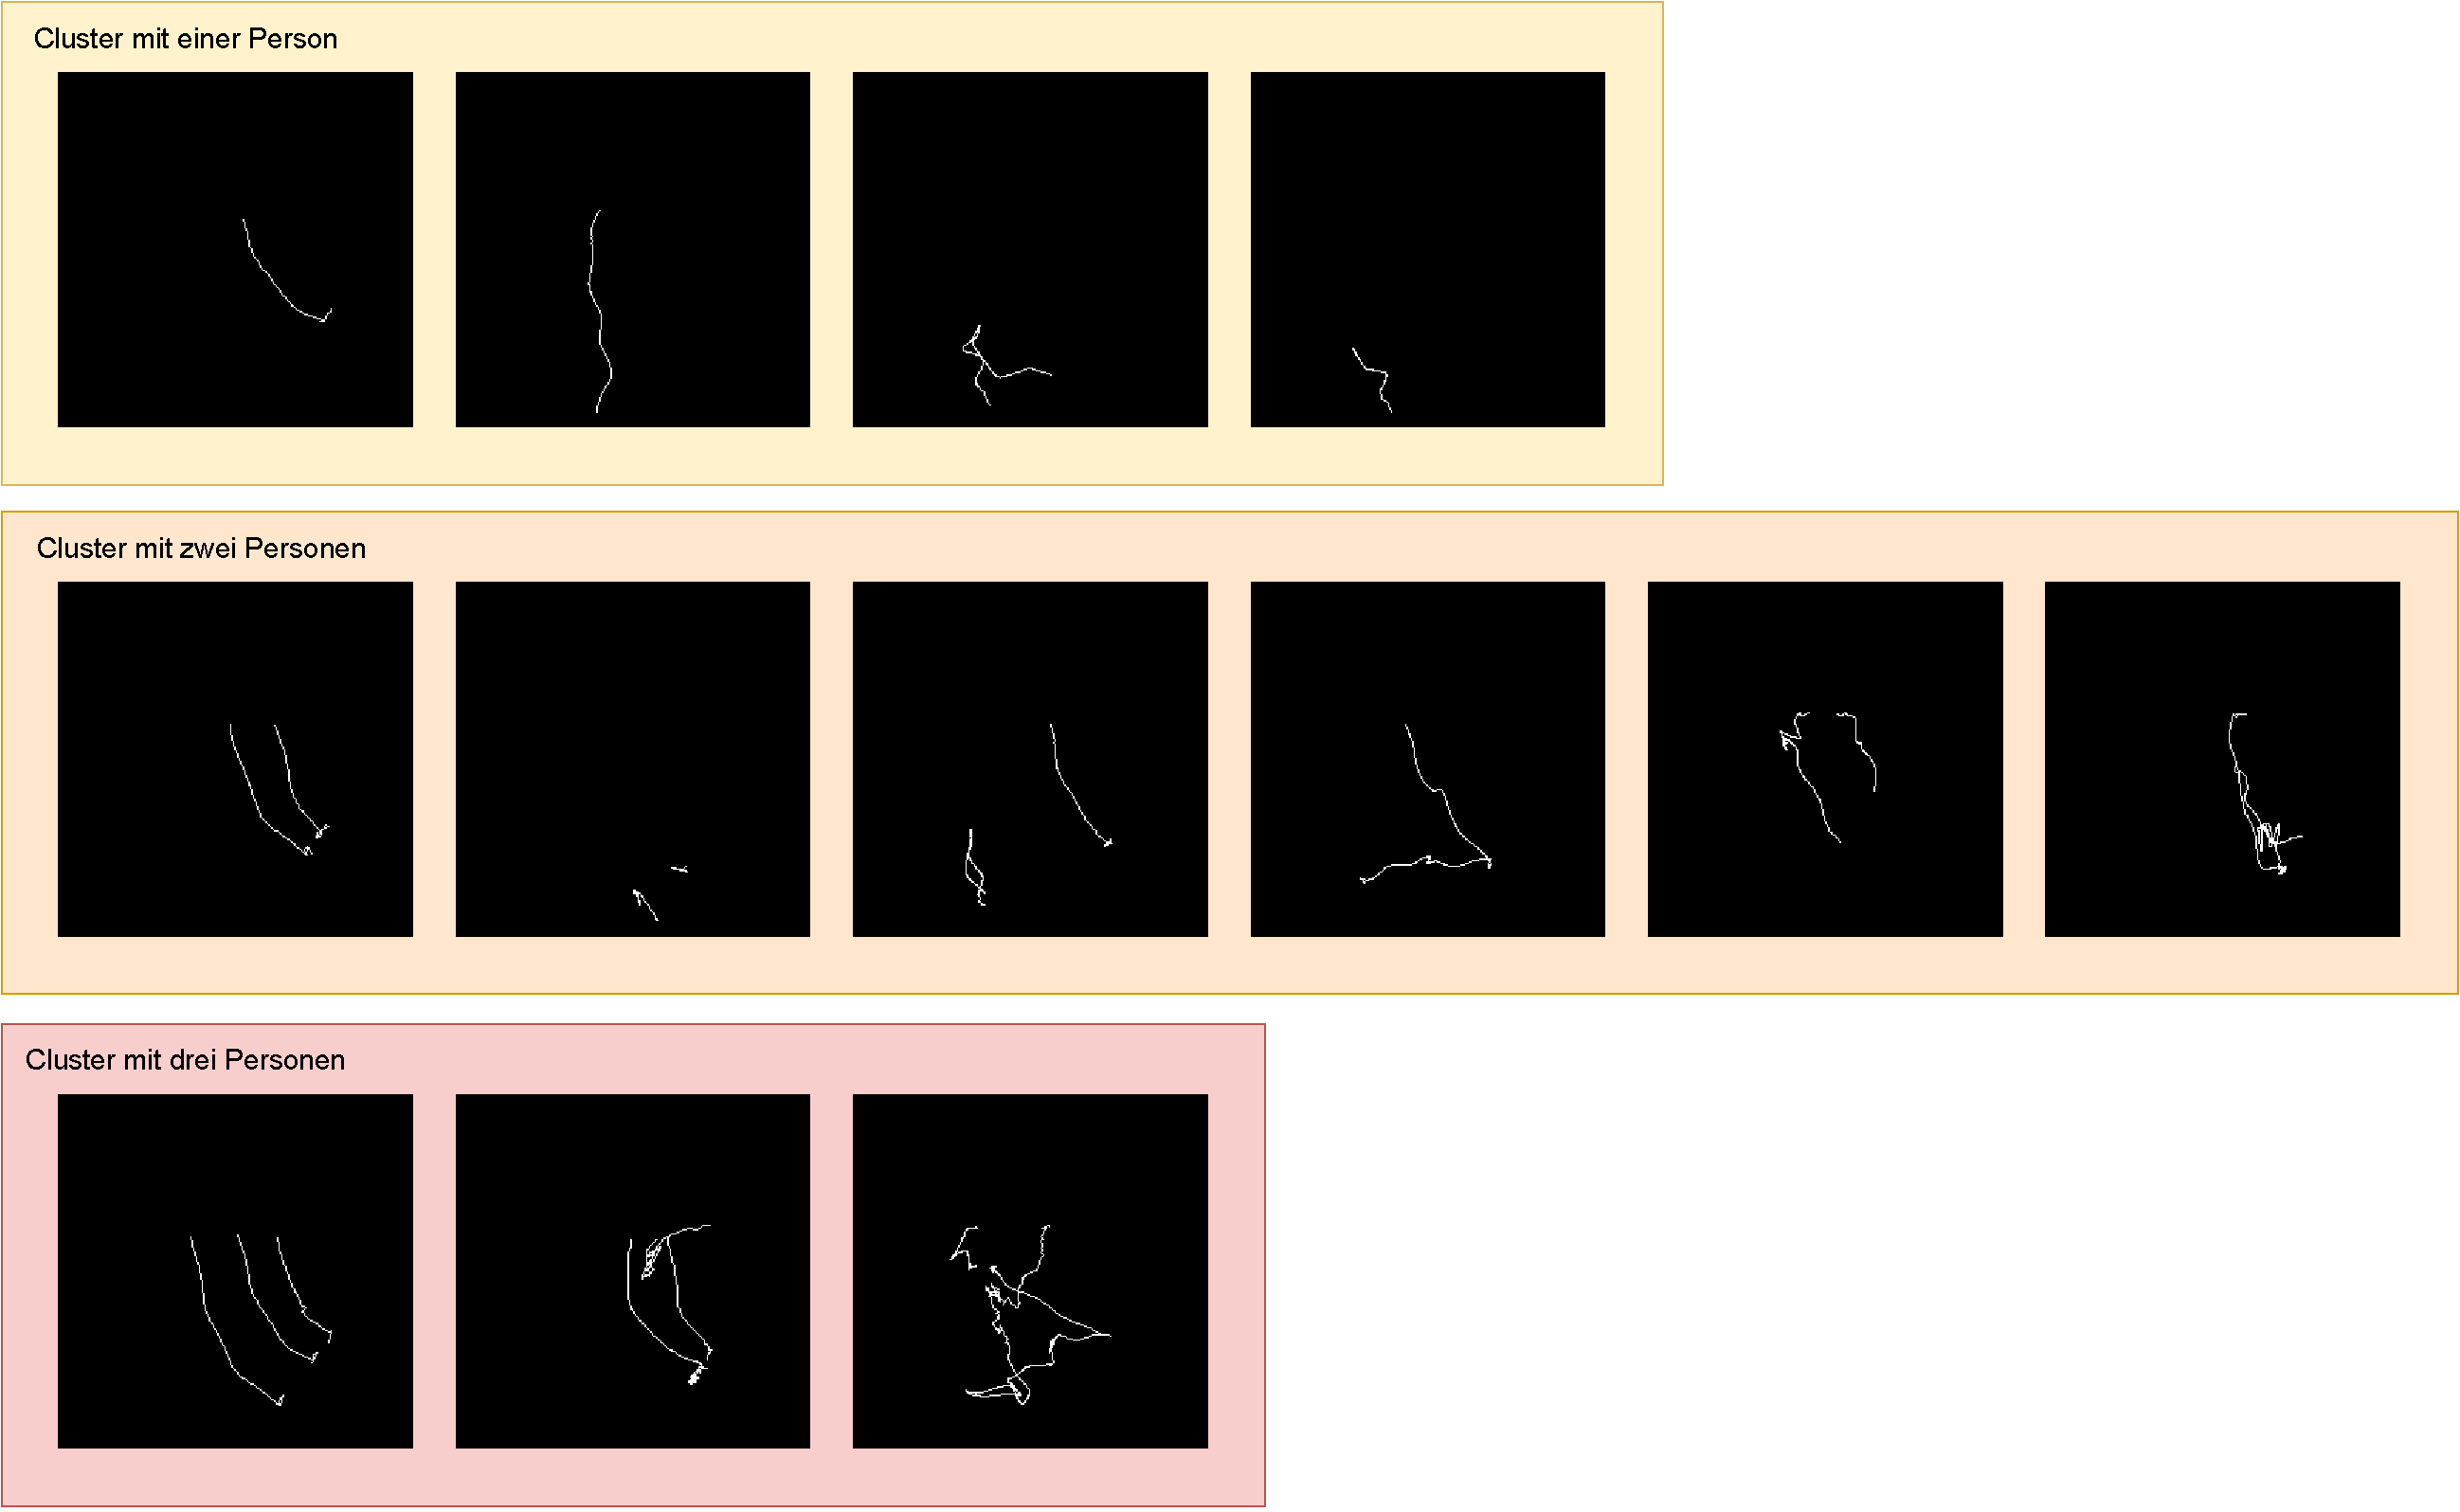
\includegraphics[width=1.2\textwidth, angle=90]{clusters.pdf}
    \end{center}
    \caption{Repräsentanten der manuell erstellten Cluster.}
    \label{fig:Clusters}
\end{figure}
Die Ergebnisse und eine sprachliche Beschreibung des Inhalts
können im Evaluation-Verzeichnis des Code-Repositories eingesehen werden.
Das hierarchische Clustering wurde mit den x- und z-Werten als Vergleichsattribute gestartet.
Der Threshold wurde dabei jeweils so gewählt,
dass genau so viele Cluster entstehen wie auch manuell erkannt wurden.
Die Auswertung zeigt, dass die vom Tool berechneten Cluster genau mit den Ground-Truth-Daten übereinstimmen.
Diese Minimalbeispiele sind aber nur bedingt aussagekräftig,
da lediglich eine kleine Teilmenge der tatsächlich vorhandenen Daten genutzt wurde.
Manche Muster treten dadurch gegebenenfalls überhaupt nicht auf.
In \autoref{6-GroundTruth} soll daher die Analyse auf mehr gefilterte Daten
für ein bis drei Personen ausgeweitet werden.
Aufgrund der Vielzahl der Daten ist das manuelle Clustering allerdings nicht so
zuverlässig möglich wie in den oben beschriebenen Minimalbeispielen.
Die Daten wurden aber nach bestem Wissen auf die wichtigsten Bewegungen hin untersucht.
Spezielle Bewegungen, die nur einmalig auftreten, wurden ignoriert.
Ziel ist es zu überprüfen,
ob häufig wiederkehrende Muster vom Tool korrekt erkannt werden.
Abschließend bleibt zu erwähnen,
dass beim Clustering von Bewegungsdaten, mithilfe von Laufwegen,
der Zweck des Gehens offen bleibt \citep{monastero_traces_2018}.
Dieser kann durch manuelle Interpretation bestimmt werden,
wobei die gefundenen Cluster unterstützend eingesetzt werden können.
Zur Automatisierung derartiger Interpretationen ist weitere Forschung notwendig.

\section{Ground-Truth-Analyse}
\label{6-GroundTruth}
Im gefilterten Datensatz mit drei Personen befinden sich insgesamt 103 Records.
Die manuelle Einteilung ergab,
dass es sich bei vielen darin vorkommenden Bewegungsabläufen
um spezielle Bewegungen, die nicht häufiger auftreten, handelt.
Sie werden im Folgenden nicht aufgeführt.
Allerdings wurde ein eindeutiges Cluster identifiziert.
\autoref{fig:3PersClust1} zeigt einen Repräsentanten dieses Clusters.
\begin{figure}[ht]
    \begin{center}
    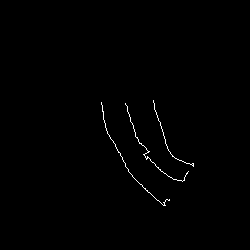
\includegraphics[width=0.15\textwidth]{representation3PersCluster1.png}
    \end{center}
    \caption{Repräsentant des nicht trivialen Clusters mit drei Personen.}
    \label{fig:3PersClust1}
\end{figure}
Es handelt sich dabei um drei Personen, die nebeneinander durch den Sensorbereich laufen.
Dieselben Erkenntnisse lieferte auch das Minimalbeispiel aus \autoref{6-Bemerkungen}.
Grund hierfür kann sein, dass die Datenmenge mit circa 100 Records immer noch gering ist.
Anschließend wurde überprüft, ob auch das Tool diese häufig auftretende Bewegung korrekt erkannt hat.
Die Ergebnisse der Berechnungen stimmen mit dem manuell gefundenen Cluster überein.
Im Wesentlichen wird nur ein nicht-triviales Cluster gefunden,
und zwar das oben beschriebene.

Die Teilmenge aller Records mit zwei Personen enthält 513 Records.
Bei der manuellen Durchsicht lassen sich wieder spezielle,
nicht wiederkehrende Bewegungen erkennen.
Diese werden erneut ignoriert.
Im Gegensatz zum Fall mit drei Personen sind hier aber mehrere häufig auftretende Bewegungen identifizierbar.
\autoref{fig:2PersClusters} zeigt jeweils einen Repräsentanten dieser manuell erkannten Muster.
\begin{figure}[ht]
    \begin{center}
    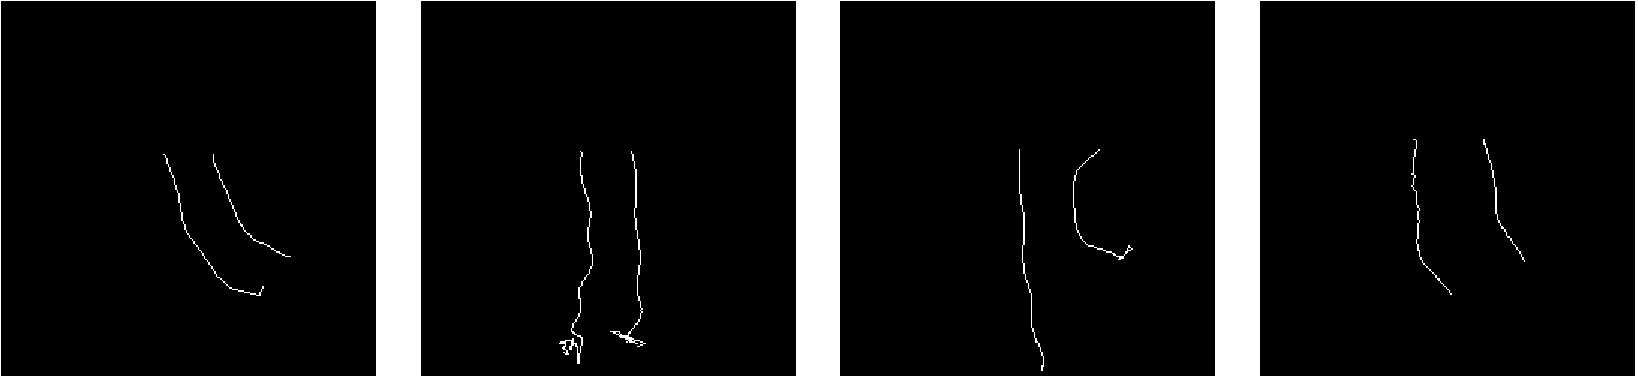
\includegraphics[width=0.65\textwidth]{2PersClusters.pdf}
    \end{center}
    \caption{Repräsentanten der größten Cluster mit zwei Personen.}
    \label{fig:2PersClusters}
\end{figure}
Zum einen handelt es sich um den Fall, dass zwei Personen durch den Aufnahmebereich laufen.
Dies ist die analoge Bewegung zum gefundenen Cluster bei drei Personen.
Der zweite Fall zeigt, wie sich zwei Personen dem Sensor nähern.
In Szenario drei bewegt sich eine Person zur Kamera,
während eine andere lediglich durch das Bild läuft.
Im letzten Fall laufen zwei Personen gemeinsam zum oberen Bildrand.
Alle Szenarien werden durch das Tool gefunden.
Bei dieser großen Menge an Records fällt auf,
dass bei niedrigen Thresholds ähnliche Records teilweise noch in unterschiedlichen Clustern liegen
und erst in späteren Schritten kombiniert werden,
da andere Szenarien noch eine höhere Ähnlichkeit aufweisen.

Das Tool kann für Datensätze mit Ein- bis Zweitausend Records effizient eingesetzt werden.
Auf einem heute typischen Mittelklasse-Heimrechner werden innerhalb weniger Minuten Ergebnisse geliefert.
Ab einigen Tausend Records nimmt die Bearbeitungszeit zu,
sodass, unter Umständen, mit mehreren Stunden Wartezeit zu rechnen ist.
Die meisten Hierarchischen Clustering-Verfahren werden den Komplexitätsklassen
\emph{O(n²)} oder \emph{O(n³)} zugeordnet.
Das implementierte Tool fällt in die Klasse \emph{O(n²)},
wie die Zeitmessungen aus \autoref{tbl:CalcTime} belegen.
Die Verdoppelung der Recordanzahl führt nicht zu einer Verachtfachung der Bearbeitungszeit,
wie dies bei \emph{O(n³)} der Fall wäre.
Die Zeit zum Einlesen der Daten
und zum Schreiben der Ergebnisse wurde hier ignoriert.
\begin{table}[ht]
  \begin{center}
  \begin{tabular}{ |c|c| } 
   \hline
   Recordanzahl & Bearbeitungszeit (Sekunden) \\
   \hline \hline
   100 & 9 \\
   \hline
   200 & 30 \\
   \hline
   400 & 133 \\
   \hline
   800 & 637 \\
   \hline
  \end{tabular}
  \caption{Bearbeitungszeiten des Clusteringvorgangs nach Recordanzahl.}
  \label{tbl:CalcTime}
  \end{center}
\end{table}
Diese Limitierung muss beachtet werden,
falls in Zukunft noch umfangreichere Datenmengen geclustert werden müssen.
In diesem Fall muss entweder ein leistungsstärkerer Rechner eingesetzt
oder das Tool weiter optimiert werden.
Mögliche Optionen sind Parallelisierung
oder die Implementierung einer effizienteren Version des Clustering-Verfahrens \citep{patel_study_2015}.

Insgesamt befinden sich 3523 Records mit einer Person im gefilterten Datensatz.
Allerdings wiederholen sich die Bewegungsmuster oft.
Deshalb soll die Analyse im Folgenden auf eine Teilmenge mit 1000 beliebigen Records eingeschränkt werden.
Erneut wird überprüft, ob wiederkehrende Bewegungen korrekt erkannt werden.
\autoref{fig:1PersClusters} zeigt jeweils einen Repräsentanten der manuell erkannten Muster.
\begin{figure}[ht]
    \begin{center}
    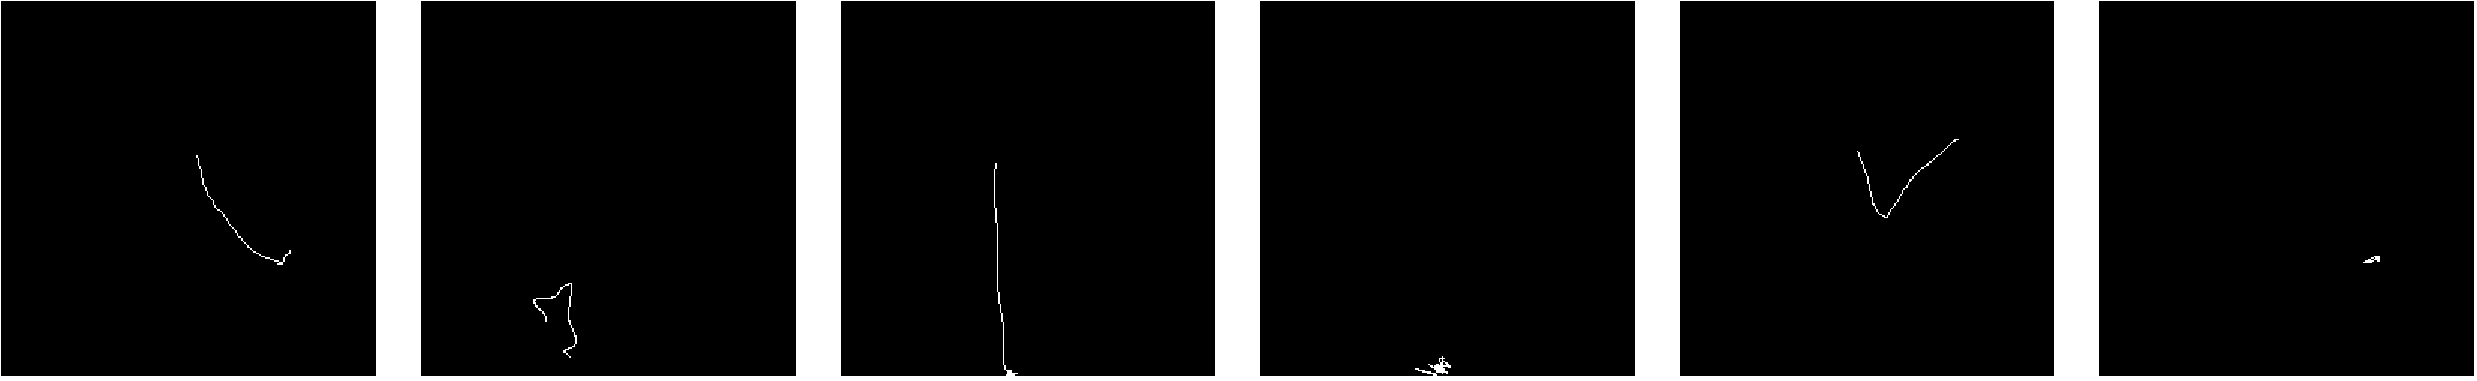
\includegraphics[width=\textwidth]{1PersClusters.pdf}
    \end{center}
    \caption{Repräsentanten der größten Cluster mit einer Person.}
    \label{fig:1PersClusters}
\end{figure}
Im ersten Fall bewegt sich eine Person durch den Aufnahmebereich,
während sie sich im zweiten Szenario unmittelbar vor der Kamera befindet.
Bild drei zeigt ein direktes Zugehen auf den Bildschirm.
Im vierten und sechsten Fall steht die Person an verschiedenen Positionen beinahe still.
Szenario fünf zeigt, wie eine Person nach vorne läuft,
sich umdreht und wieder zurückläuft.
All diese Fälle können durch das Tool erkannt werden.
Zu erwähnen ist allerdings, dass manche Cluster bei hohen Thresholds bereits in andere Gruppen integriert werden.
So kann etwa das fünfte Szenario nur bei niedrigeren Thresholds erkannt werden,
während es bei höheren Werten unter Umständen bereits mit Cluster eins zusammengeführt wurde.
Dies verdeutlicht erneut, dass eine sinnvolle Suche nach Clustern möglich ist,
diese aber dennoch manuell betrachtet werden müssen.
Dabei sollte auch mit verschiedenen Thresholds experimentiert werden.

Die Auswertung des gesamten Datensatzes bestätigt demnach die Vermutung der Minimalbeispiele.
Das Tool kann erfolgreich genutzt werden, um sinnvolle Cluster auf den Kinect-Bewegungsdaten zu finden.
Im folgenden Abschnitt soll abschließend die Güte der gefundenen Cluster an einigen Beispielen
überprüft werden.

\section{Statistische Analyse}
\label{6-Statistical}
Abschließend soll mithilfe von deskriptiven Statistiken überprüft werden,
ob ein Zusammenhang zwischen den Record-Bestandteilen eines Clusters besteht.
Der Grad der Übereinstimmung liefert Informationen zur Ähnlichkeit.
Konkret werden nun für die Komponenten einiger Cluster
die Standardabweichung, der Mittelwert, das Maximum und das Minimum für die x-Laufwege berechnet
und tabellarisch dargestellt.
In der letzten Zeile ist jeweils die Standardabweichung aller darüberstehenden Werte aufgeführt.
Hier werden teilweise die Minimalbeispiele aus \autoref{6-GroundTruth} mit veränderten Thresholds wieder aufgegriffen.
Auch diese Daten befinden sich im Evaluation-Verzeichnis des Code-Repositories.
Zunächst wird das erste Cluster mit drei Personen betrachtet (\autoref{fig:Clusters}).
Die Ergebnisse werden in \autoref{tbl:ClustThreePers} dargestellt
und sind auf zwei Nachkommastellen gerundet.
Anschließend werden die Werte des ersten Clusters mit zwei Personen aus \autoref{fig:Clusters} berechnet.
Sie sind in \autoref{tbl:ClustTwoPers} zu sehen.
Wird im selben Beispiel der Threshold noch höher gesetzt,
sodass die gefundenen Cluster augenscheinlich nicht mehr sinnvoll sind,
werden die Werte in \autoref{tbl:ClustTwoPersHighThreshold} geliefert.
\begin{table}[ht]
  \begin{center}
    \begin{tabular}{ |c|c|c|c|c| } 
      \hline
      Record & Minimum & Maximum & Mittelwert & Standardabw. \\
      \hline \hline
      2017-05-04 16.35.15.463 & -2.12 & 0.63 & -0.59 & 0,72 \\
      \hline
      2017-04-13 12.34.38.535 & -1.72 & 0.46 & -0.65 & 0,58 \\
      \hline
      2017-05-08 12.30.56.954 & -2.09 & 0.12 & -1.01 & 0.56 \\
      \hline
      2017-04-13 12.36.06.669 & -1.83 & 0.43 & -0.70 & 0.57 \\
      \hline
      2017-04-20 12.35.56.578 & -2.06 & 0.50 & -0.75 & 0.67 \\
      \hline
      2017-04-10 11.53.16.991 & -2.09 & -0.61 & -1.15 & 0.36 \\
      \hline
      2017-05-08 12.45.55.652 & -1.84 & 0.51 & -0.64 & 0.65 \\
      \hline
      2017-04-06 09.47.43.189 & -1.96 & 0.44 & -0.66 & 0.64 \\
      \hline
      2017-04-05 13.00.04.745 & -1.79 & 0.17 & -0.79 & 0.50 \\
      \hline
      2017-04-11 13.29.55.196 & -2.06 & 0.72 & -0.47 & 0.72 \\
      \hline
      2017-04-07 13.19.05.395 & -2.01 & 0.32 & -0.81 & 0.56 \\
      \hline
      2017-04-21 14.17.23.301 & -2.03 & 0.30 & -0.91 & 0.59 \\
      \hline
      2017-04-26 11.59.37.413 & -1.74 & 0.31 & -0.76 & 0.55 \\
      \hline
      2017-04-21 12.58.27.894 & -1.84 & 0.20 & -0.81 & 0.51 \\
      \hline
      2017-04-19 12.54.19.390 & -1.81 & 0.66 & -0.54 & 0.69 \\
      \hline
      2017-04-27 12.36.45.995 & -1.85 & -0.04 & -0.92 & 0.50 \\
      \hline
      2017-05-04 13.13.17.884 & -2.07 & -0.03 & -0.85 & 0.52 \\
      \hline
      2017-04-05 09.28.25.562 & -1.78 & 0.36 & -0.66 & 0.58 \\
      \hline
      2017-05-04 13.24.36.117 & -2.00 & 0.38 & -0.66 & 0.65 \\
      \hline
      2017-04-05 13.01.44.147 & -2.20 & 0.41 & -0.73 & 0.63 \\
      \hline
      2017-04-07 11.05.51.351 & -1.89 & 0.32 & -0.63 & 0.65 \\
      \hline
      \hline
      Standardabweichung & 0.14 & 0.29 & 0.16 & 0.09 \\
      \hline
    \end{tabular}
    \caption{Deskriptive Statistiken für das Cluster mit drei Personen.}
    \label{tbl:ClustThreePers}
  \end{center}
\end{table}
  \begin{table}[ht]
    \begin{center}
      \begin{tabular}{ |c|c|c|c|c| } 
        \hline
        Record & Minimum & Maximum & Mittelwert & Standardabw. \\
        \hline \hline
        2017-04-06 12.26.06.199 & -1.90 & -0.34 & -0.98 & 0,49 \\
        \hline
        2017-04-05 09.13.53.631 & -1.73 & 0.01 & -0.88 & 0,41\\
        \hline
        2017-04-04 16.54.30.868 & -1.67 & 0.45 & -0.61 & 0.61 \\
        \hline
        2017-04-05 12.32.59.075 & -1.71 & 0.30 & -0.62 & 0.54 \\
        \hline
        2017-04-05 12.53.33.743 & -1.80 & 0.28 & -0.67 & 0.55 \\
        \hline
        2017-04-05 10.03.28.598 & -1.89 & -0.02 & -1.00 & 0.51 \\
        \hline
        2017-04-05 08.16.53.128 & -1.77 & -0.03 & -0.88 & 0.48 \\
        \hline
        2017-04-05 14.44.27.088 & -1.87 & 0.31 & -0.72 & 0.60 \\
        \hline
        2017-04-06 12.31.41.933 & -1.77 & 0.28 & -0.70 & 0.61 \\
        \hline
        2017-04-05 15.01.29.988 & -1.95 & 0.58 & -0.50 & 0.68 \\
        \hline
        2017-04-04 17.27.46.240 & -1.93 & -0.32 & -1.10 & 0.38 \\
        \hline
        2017-04-05 15.02.00.252 & -2.13 & 0.26 & -0.83 & 0.65 \\
        \hline
        2017-04-05 17.08.48.758 & -1.76 & 0.30 & -0.73 & 0.64 \\
        \hline
        2017-04-05 16.59.22.830 & -1.92 & 0.38 & -0.74 & 0.57 \\
        \hline
        2017-04-05 11.40.51.237 & -1.32 & 0.17 & -0.49 & 0.46 \\
        \hline
        2017-04-06 11.38.42.632 & -1.67 & 0.12 & -0.81 & 0.50 \\
        \hline
        2017-04-05 10.56.51.141 & -1.77 & 0.31 & -0.68 & 0.58 \\
        \hline
        2017-04-05 12.29.05.007 & -1.85 & 0.16 & -0.80 & 0.55 \\
        \hline
        2017-04-05 13.33.56.412 & -1.97 & 0.31 & -0.79 & 0.63 \\
        \hline
        2017-04-05 10.59.42.469 & -1.77 & -0.17 & -0.92 & 0.49 \\
        \hline
        \hline
        Standardabweichung & 0.16 & 0.24 & 0.16 & 0.08 \\
        \hline
       \end{tabular}
    \caption{Deskriptive Statistiken für das Cluster mit zwei Personen.}
    \label{tbl:ClustTwoPers}
  \end{center}
\end{table}
\begin{table}[ht]
  \begin{center}
    \begin{tabular}{ |c|c|c|c|c| } 
      \hline
      Record & Minimum & Maximum & Mittelwert & Standardabw. \\
      \hline \hline
      2017-04-06 12.26.06.199 & -1.90 & -0.34 & -0.98 & 0,49 \\
      \hline
      2017-04-05 09.13.53.631 & -1.73 & 0.01 & -0.88 & 0,41\\
      \hline
      2017-04-04 16.54.30.868 & -1.67 & 0.45 & -0.61 & 0.61 \\
      \hline
      2017-04-05 12.32.59.075 & -1.71 & 0.30 & -0.62 & 0.54 \\
      \hline
      2017-04-04 18.04.06.507 & -1.23 & 1.07 & -0.14 & 0.54 \\
      \hline
      2017-04-05 12.53.33.743 & -1.80 & 0.28 & -0.67 & 0.55 \\
      \hline
      2017-04-05 10.03.28.598 & -1.89 & -0.02 & -1.00 & 0.51 \\
      \hline
      2017-04-05 08.16.53.128 & -1.77 & -0.03 & -0.88 & 0.48 \\
      \hline
      2017-04-05 12.40.57.142 & -1.52 & -0.23 & -1.00 & 0.22 \\
      \hline
      2017-04-05 14.44.27.088 & -1.87 & 0.31 & -0.72 & 0.60 \\
      \hline
      2017-04-06 12.31.41.933 & -1.77 & 0.28 & -0.70 & 0.61 \\
      \hline
      2017-04-05 15.01.29.988 & -1.95 & 0.58 & -0.50 & 0.68 \\
      \hline
      2017-04-04 17.27.46.240 & -1.93 & -0.32 & -1.10 & 0.38 \\
      \hline
      \textbf{2017-04-04 14.55.11.727} & \textbf{-1.57} & \textbf{1.02} & \textbf{0.36} & \textbf{0.84} \\
      \hline
      2017-04-05 15.02.00.252 & -2.13 & 0.26 & -0.83 & 0.65 \\
      \hline
      2017-04-05 17.08.48.758 & -1.76 & 0.30 & -0.73 & 0.64 \\
      \hline
      2017-04-05 16.59.22.830 & -1.92 & 0.38 & -0.74 & 0.57 \\
      \hline
      2017-04-05 11.40.51.237 & -1.32 & 0.17 & -0.49 & 0.46 \\
      \hline
      2017-04-05 11.41.21.472 & -1.08 & -0.14 & -0.53 & 0.36 \\
      \hline
      2017-04-06 11.38.42.632 & -1.67 & 0.12 & -0.81 & 0.50 \\
      \hline
      2017-04-05 10.56.51.141 & -1.77 & 0.31 & -0.68 & 0.58 \\
      \hline
      2017-04-05 12.29.05.007 & -1.85 & 0.16 & -0.80 & 0.55 \\
      \hline
      2017-04-05 13.33.56.412 & -1.97 & 0.31 & -0.79 & 0.63 \\
      \hline
      2017-04-05 10.59.42.469 & -1.77 & -0.17 & -0.92 & 0.49 \\
      \hline
      \hline
      Standardabweichung & 0.24 & 0.35 & 0.31 & 0.12 \\
      \hline
     \end{tabular}
    \caption{Deskriptive Statistiken für das Cluster mit zwei Pers. (hoher Threshold).}
    \label{tbl:ClustTwoPersHighThreshold}
  \end{center}
\end{table}
Die Mittelwerte und Standardabweichungen in den ersten beiden Beispielen
bewegen sich jeweils in einem ähnlichen Rahmen.
Auch die Standardabweichung dieser Werte ist mit \emph{0.16} und \emph{0.09} im ersten,
sowie \emph{0.16} und \emph{0.08} im zweiten überprüften Cluster gering.
Dadurch wird bestätigt, dass die Records einen inhaltlichen Zusammenhang aufweisen.
Beim dritten Fall hingegen schwanken diese Werte stärker.
Die ermittelte Gesamtstandardabweichungen sind mit \emph{0.31} und \emph{0.12} um
circa 52 Prozent, bzw. 39 Prozent höher als bei den zuerst betrachteten Clustern.
Einige Records scheinen also nicht in die Gruppe zu passen.
So weicht beispielsweise die Zeile \emph{2017-04-04 14.55.11.727} stark von den anderen ab.
Ein Blick in die Visualisierung bestätigt,
dass dieser Laufweg nicht zu den anderen passt.
Dieser Fall wurde lediglich aufgrund des zu hohen Thresholds einsortiert.
Dies betont einerseits erneut die bedeutende Rolle eines geeigneten Thresholds
und andererseits, dass die Bestimmung der Güte mittels deskriptiver Statistiken möglich ist.
Die Records der Cluster der beiden ersten Beispiele weisen eine hohe Ähnlichkeit auf.
Mithilfe des entwickelten Tools ist folglich ein sinnvolles Clustering möglich.
Beim letzten Cluster sind durch einen hohen Threshold hingegen zu viele Records zusammengeführt worden.
    \chapter{Fazit}
\label{chapter7}
Im Rahmen des \emph{HoPE-Projekts} wird das Verhalten von Menschen
bei der Nutzung von interaktiven Wandbildschirmen analysiert.
Dazu muss ein methodisches Rahmenwerk entwickelt werden, welches eine auf Sensordaten-basierende,
automatische und zeitlich uneingeschränkte Evaluation von Ambient Displays ermöglicht \citep{unibw_honeypot-effekt_2021}.
Bewegungsdaten von Tiefenkameras können genutzt werden,
um das Verhalten von Menschen vor Wandbildschirmen zu analysieren.
Es kann versucht werden, ob sich Kategorien identifizieren lassen,
die etwas über das Verhalten von Menschen vor Wandbildschirmen aussagen.
Bei großen Datensätzen ist eine manuelle Identifikation nicht möglich.
Daher ist eine Automatisierung notwendig.
Diese Bachelorarbeit ist ein Beitrag zum Rahmenwerk für die Evaluation.
Wesentliches Ziel war die Implementierung eines Systems zur Kategorisierung von vorliegenden \emph{Kinect-Bewegungsdaten}.
Das Problem wurde mithilfe von deterministischen Algorithmen gelöst.
Konkret kam \emph{hierarchisches Clustering} mithilfe des \emph{\ac{DTW}} Algorithmus zum Einsatz,
da diese Algorithmen für den Umgang mit \ac{TSD} geeignet sind.
In der Evaluation wurde die Praxistauglichkeit des Tools überprüft.
Dazu wurden gefilterte Teilmengen des vorliegenden Datensatzes geclustert.
Dabei hat sich gezeigt, dass die Rolle eines geeigneten Thresholds von Bedeutung ist.
Die durchgeführte Ground-Truth-Analyse bestätigt, dass ein sinnvolles Clustering möglich ist.
Die deskriptiven Statistiken belegen zudem, dass die Qualität der gefunden Cluster hoch ist.
Mit den genutzten Algorithmen lassen sich Bewegungsdaten also ohne Vorwissen clustern.
Zu erwähnen ist allerdings, dass beim Clustering von Bewegungsdaten
der Zweck der Bewegung offen bleibt \citep{monastero_traces_2018}.
Dieser kann durch manuelle Interpretation bestimmt werden.
Zur Automatisierung dieses Schritts ist weitere Forschung notwendig.
In zukünftigen Arbeiten kann außerdem versucht werden die Effizienz des Tools weiter zu erhöhen,
um die Nutzbarkeit bei großen Datensätzen zu steigern.
Zudem ist der Einsatz anderer Distanzfunktionen denkbar.
Abhängig von den Daten können mit anderen Funktionen gegebenenfalls die Ergebnisse verbessert werden.
Des Weiteren können in künftigen Forschungsarbeiten, mithilfe der Anwendung, weitere Datenanalysen stattfinden.

% ---------------------------------------------------------------
\backmatter
    \chapter{Abkürzungsverzeichnis}
\begin{acronym}[BT Classic]
    \acro{fps}{frames per second}
    \acro{HCI}{Mensch-Computer-Interaktion}
    \acro{RGB}{Rot-Grün-Blau}
    \acro{ToF}{Time-of-Flight}
    \acro{DTW}{Dynamich Time Warping}
    \acro{TSD}{Time-Series Data}
\end{acronym}
    \listoffigures
    \begingroup
        \hbadness 10000
        \linespread{1.2}
        \renewcommand*{\bibfont}{\small}
        \setlength\bibhang{2em}
        \printbibliography
    \endgroup
    \begingroup
        \hbadness 10000
        \newpage

\thispagestyle{empty}

\begin{large}

\vspace*{2cm}

\noindent
Hiermit versichere ich, die vorliegende Arbeit selbständig und ohne fremde Hilfe verfasst,
die Zitate ordnungsgemäß gekennzeichnet und keine anderen,
als die im Literatur/Schriftenverzeichnis angegebenen Quellen und Hilfsmittel benutzt zu haben.\\[1em]

\noindent
Ferner habe ich vom Merkblatt über die Verwendung von studentischen Abschlussarbeiten Kenntnis genommen
und räume das einfache Nutzungsrecht an meiner Bachelorarbeit der Universität der Bundeswehr München ein.

\vspace{2cm}

\noindent
München, den 31. Mai 2022

\vspace{3cm}

\hspace*{7cm}
\dotfill\\
\hspace*{10cm}
\textit{(Unterschrift)}

\end{large}

    \endgroup

\end{document}
